\chapter{初值问题的数值求解}
\label{chap:ode-numerical-methods}

考虑初值问题$\dot{x}=x(1-x)$，$x(0)=0.2$，我们想知道$x(1)$是多少。这个方程恰好能分离变量，答案是$\mathrm{e}/(\mathrm{e}+4)\approx0.404610$。可是只要右端稍微复杂一点，比如添上一项$\sin(tx)$，第~\ref{chap:ordinary-differential-equations}章的解法就用不上了。第~\ref{chap:ode-existence-continuation}章的定理告诉我们解存在且唯一，却没有告诉我们它在$t=1$时等于多少。

计算机只能保存有限个数、做有限次运算，所以真正能算的是解曲线上有限个时刻的近似值。把曲线换成一串数之后，马上面临三个问题：从一个时刻到下一个时刻究竟怎样走；每一步的小偏差累积到终点时有多大；步长由什么决定，能不能让程序自己选。

本章按这三个问题展开。前三节建立时间离散的语言，再给出Euler方法和Runge--Kutta方法，用同一个初值问题比较它们的误差与计算量。第~\ref{sec:odenum-error-convergence}节在有限区间上证明，一步误差经过怎样的条件才累积成确定阶数的全局误差。

高阶方法并不总是最好的选择。第~\ref{sec:odenum-stiff}节的快慢系统里，真正限制步长的是数值扰动的稳定性，而不是精度，这引出了隐式方法。第~\ref{sec:odenum-adaptive}节让程序按局部误差估计自动调节步长，并说明这样的估计能保证什么、不能保证什么。

本章始终讨论有限时间区间，并假定真解在整个区间上存在。上面的方程$\dot{x}=x(1-x)$贯穿全章：它是非线性的，手算只需几位小数，又有闭式解可以用来核对结果。

\section{时间离散}
\label{sec:odenum-time-discretization}

连续的解是一条曲线，算法只能交出有限个数。这有限个数应该是什么，怎样一个接一个地产生，又该拿什么标准评价它们？

\paragraph{时间网格与一步更新}
固定初值问题
\begin{equation}
 \dot{\bm{x}}(t)=\bm{f}(t,\bm{x}(t)),\qquad \bm{x}(t_0)=\bm{x}_0,
 \label{eq:odenum-ivp}
\end{equation}
并假定它在有限区间$[t_0,t_0+T]$上有唯一解$\bm{x}(t)$，$\bm{x}(t)\in\mathbb{R}^{n}$。存在、唯一与延拓的条件见第~\ref{chap:ode-existence-continuation}章。

把区间等分成$N$份，步长$h=T/N$，得到\term{时间网格}（time grid）
\begin{equation}
 t_k=t_0+kh,\qquad k=0,1,\ldots,N.
 \label{eq:odenum-grid}
\end{equation}
数值解是一串向量$\bm{x}^{(0)},\bm{x}^{(1)},\ldots,\bm{x}^{(N)}$，其中$\bm{x}^{(k)}$用来近似$\bm{x}(t_k)$。上标带括号表示网格编号，不是导数的阶数。

真解自身满足一个“一步”关系。在$[t_k,t_{k+1}]$上积分方程，得到
\begin{equation}
 \bm{x}(t_{k+1})=\bm{x}(t_k)+\int_{t_k}^{t_{k+1}}\bm{f}(s,\bm{x}(s))\,\mathrm{d}s.
 \label{eq:odenum-integral-step}
\end{equation}
右端的积分依赖这一步内部尚不知道的解，所以不能直接算。本章所有方法都在回答同一件事：只用当前已知的量，怎样近似这个积分。

用流映射的话说，式~\eqref{eq:odenum-integral-step}就是
\[
 \bm{x}(t_{k+1})=\bm{\varphi}_{t_k,t_{k+1}}\bigl(\bm{x}(t_k)\bigr),
\]
其中$\bm{\varphi}_{s,t}(\bm{y})$表示时刻$s$从$\bm{y}$出发的解在时刻$t$的值。流映射一般算不出来，于是用一个可计算的映射代替它。

\begin{definition}[一步方法]
 \label{def:odenum-one-step}
 \term{一步方法}（one-step method）由一族映射$\bm{\Psi}_h(t,\cdot)$给出，步长为$h$时按
 \begin{equation}
  \bm{x}^{(k+1)}=\bm{\Psi}_h\bigl(t_k,\bm{x}^{(k)}\bigr),\qquad k=0,1,\ldots,N-1
  \label{eq:odenum-one-step}
 \end{equation}
 从$\bm{x}^{(0)}$逐步计算。$\bm{\Psi}_h$只依赖当前的$t_k$、$\bm{x}^{(k)}$、步长和右端$\bm{f}$，不依赖更早的网格值。
\end{definition}

\paragraph{连续曲线、网格值与插值结果}
离散之后手里有三种不同的对象，它们很容易被混为一谈。图~\ref{fig:odenum-grid-values}把它们画在一起：蓝线是真解，是我们想知道却拿不到的函数；绿点是网格值，是算法实际产生的全部输出；绿色虚线是把相邻网格值连起来的折线，它是另加的一条规则，并不来自方程。

\begin{BookInlineFigure}
 \centering
 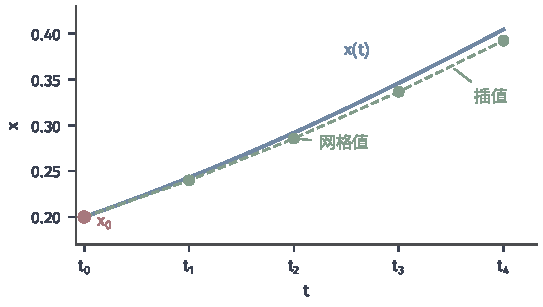
\includegraphics[width=92mm]{figures/06-differential-equations/01-ordinary-differential-equations/matplotlib/odenum-grid-values/figure.pdf}
 \caption{初值问题$\dot{x}=x(1-x)$，$x(0)=0.2$的三种对象。蓝线是真解，红点是初值，绿点是某个一步方法在步长$h=1/4$下给出的网格值，绿色虚线是对网格值作的分段线性插值。}
 \label{fig:odenum-grid-values}
\end{BookInlineFigure}

讨论误差时必须先说清比较的是哪一种对象。本章的误差都指网格点上$\bm{x}^{(k)}$与$\bm{x}(t_k)$的差。

网格点之间的值需要另外的插值规则，插值规则有自己的误差。若方法在网格上很精确，而插值只用分段线性，那么网格点之间的误差由插值决定，只有$h^2$的量级，精确的网格值也就白费了。

\paragraph{三种误差的来源}
数值解离真解有多远，来自三个不同的环节。第一，出发点可能不准：$0.2$在二进制中是无限循环小数，存进计算机时已经有舍入，初值本身也可能来自测量。第二，一步更新只是对式~\eqref{eq:odenum-integral-step}的近似。第三，每一步的运算有舍入误差，隐式方法（第~\ref{sec:odenum-stiff}节）还要加上内部方程没有解到底的误差。

用$\bm{\delta}^{(0)}$记初值误差，用$\bm{\delta}^{(k)}$（$k\geq1$）记第$k$步的计算误差，把实际算出的序列写成
\begin{equation}
 \bm{x}^{(0)}=\bm{x}_0+\bm{\delta}^{(0)},\qquad
 \bm{x}^{(k+1)}=\bm{\Psi}_h\bigl(t_k,\bm{x}^{(k)}\bigr)+\bm{\delta}^{(k+1)}.
 \label{eq:odenum-computed}
\end{equation}
理想算术且初值精确时，所有$\bm{\delta}^{(k)}$都为零。

第二个环节需要单独定义。关键是把出发点放在真解上，这样它只反映更新规则本身的缺陷，不混入以前积累的偏差。

\begin{definition}[局部截断误差与全局误差]
 \label{def:odenum-errors}
 设$\bm{x}(t)$是式~\eqref{eq:odenum-ivp}的解。第$k+1$步的\term{局部截断误差}（local truncation error）是从真解出发走一步与真解的差，
 \begin{equation}
  \bm{\ell}^{(k+1)}=\bm{\Psi}_h\bigl(t_k,\bm{x}(t_k)\bigr)-\bm{x}(t_{k+1}).
  \label{eq:odenum-local-error}
 \end{equation}
 \term{全局误差}（global error）是实际算出的网格值与真解的差，
 \begin{equation}
  \bm{e}^{(k)}=\bm{x}^{(k)}-\bm{x}(t_k).
  \label{eq:odenum-global-error}
 \end{equation}
\end{definition}

注意$\bm{\ell}^{(k+1)}$没有除以步长，它就是一步之内产生的偏差。两种误差的关系可以直接写出来。把式~\eqref{eq:odenum-computed}代入$\bm{e}^{(k+1)}$，再加减$\bm{\Psi}_h(t_k,\bm{x}(t_k))$，得到
\begin{equation}
 \bm{e}^{(k+1)}
 =\underbrace{\bm{\Psi}_h\bigl(t_k,\bm{x}^{(k)}\bigr)-\bm{\Psi}_h\bigl(t_k,\bm{x}(t_k)\bigr)}_{\text{旧误差的传播}}
 +\bm{\ell}^{(k+1)}+\bm{\delta}^{(k+1)}.
 \label{eq:odenum-error-split}
\end{equation}
每步的全局误差等于“上一步误差被更新规则放大或缩小的结果”，加上本步新产生的截断误差和计算误差。图~\ref{fig:odenum-three-errors}画出了这三个环节的位置。

\begin{BookInlineFigure}
 \centering
 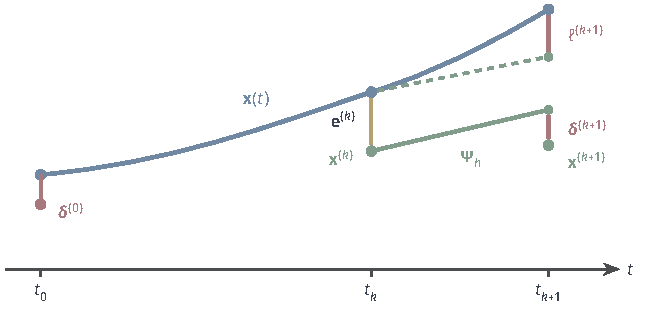
\includegraphics[width=109mm]{figures/06-differential-equations/01-ordinary-differential-equations/tikz/odenum-three-errors/figure.pdf}
 \caption{误差分解的一步。蓝线是真解，红点标出初值误差$\bm{\delta}^{(0)}$；在$t_{k+1}$处，从真解点$\bm{x}(t_k)$按规则$\bm{\Psi}_h$走一步，落点与真解之差是局部截断误差$\bm{\ell}^{(k+1)}$；从算出的$\bm{x}^{(k)}$走一步（绿色），旧误差$\bm{e}^{(k)}$被传播，再叠加计算误差$\bm{\delta}^{(k+1)}$后得到$\bm{x}^{(k+1)}$。}
 \label{fig:odenum-three-errors}
\end{BookInlineFigure}

\paragraph{残差不能代替误差}
既然真解满足方程，一个诱人的检验是把近似解代回方程，看方程满足得好不好。这种检验要分两种情况看。

如果代入的是离散格式本身，得到的永远是零。网格值正是按式~\eqref{eq:odenum-one-step}算出来的，无论$h$多大，它都严格满足自己的递推，所以离散方程的残差不提供任何信息。

如果代入的是连续的插值函数$\tilde{\bm{x}}(t)$，就可以定义\term{残差}（residual）
\[
 \bm{r}(t)=\dot{\tilde{\bm{x}}}(t)-\bm{f}\bigl(t,\tilde{\bm{x}}(t)\bigr).
\]
残差小说明$\tilde{\bm{x}}$是一个“被轻轻推过的方程”的解，但两个方程的解相差多少，取决于方程本身怎样放大扰动。

下面的两个方程真解都是$\cos t$，只差一个符号。取$\sigma=\pm5$，初值问题为
\[
 \dot{x}=\sigma(x-\cos t)-\sin t,\qquad x(0)=1.
\]
设近似函数$\tilde{x}$从同一初值出发，残差恒为$r=10^{-3}$。

记$d(t)=\tilde{x}(t)-\cos t$，两式相减得到关于差的方程：
\[
 \dot{d}=\sigma d+r,\qquad d(0)=0.
\]
解这个常系数线性方程，得到
\[
 d(t)=\frac{r}{\sigma}\bigl(\mathrm{e}^{\sigma t}-1\bigr).
\]

当$t=2$时，$\sigma=-5$给出$\lvert d\rvert\approx2\times10^{-4}$，比残差还小。$\sigma=5$给出$\lvert d\rvert\approx4.4$，是解本身量级的好几倍。图~\ref{fig:odenum-residual-gap}展示了这一差别：残差完全相同，误差相差四个多数量级。

\begin{BookInlineFigure}
 \centering
 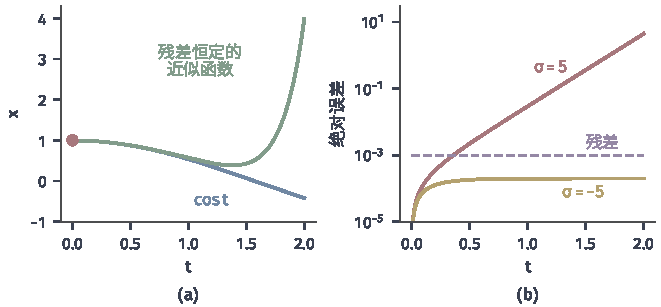
\includegraphics[width=112mm]{figures/06-differential-equations/01-ordinary-differential-equations/matplotlib/odenum-residual-gap/figure.pdf}
 \caption{残差相同而误差不同。(a)$\sigma=5$时，蓝线为真解$\cos t$，绿线为残差恒为$10^{-3}$的近似函数，二者很快分开。(b)绝对误差的对数图：紫色虚线是残差，红线和黄线分别是$\sigma=5$与$\sigma=-5$时的误差$\lvert d(t)\rvert$。}
 \label{fig:odenum-residual-gap}
\end{BookInlineFigure}

所以评价数值解时，要把初值误差、一步截断误差和每步计算误差分别记录，再结合误差的传播规律估计全局误差。这正是后面各节要做的事，传播规律由第~\ref{sec:odenum-error-convergence}节给出。


\section{Euler方法}
\label{sec:odenum-euler}

式~\eqref{eq:odenum-integral-step}的积分里，被积函数在这一步内部未知。最朴素的办法是假装它在这一步内不变，取起点的值。这样得到的方法是什么样，一步偏差多大，走完整个区间又要算多少次？

\paragraph{主要思想}
方向场在每个点$(t,\bm{x})$上给出一个速度$\bm{f}(t,\bm{x})$。站在当前点，读一次速度，沿这个方向走$h$的时间，到达新位置后再读一次，这就是\term{显式Euler方法}（explicit Euler method）。它像顺水漂流时每隔一段时间才看一眼水流方向：两次观察之间，方向按上一次的读数保持不变。类比的界限在于：真实的漂流者一直被水流带动，折线在两次读数之间却完全不看水流。

积分的说法与此相同。用$\bm{f}(t_k,\bm{x}^{(k)})$代替式~\eqref{eq:odenum-integral-step}中的被积函数，积分变成长度$h$乘以这个常向量，得到
\begin{equation}
 \bm{x}^{(k+1)}=\bm{x}^{(k)}+h\,\bm{f}\bigl(t_k,\bm{x}^{(k)}\bigr).
 \label{eq:odenum-euler}
\end{equation}

“显式”是指新值已经写在等号左边，右端只用旧值，代入即得。图~\ref{fig:odenum-euler-polygon}是这样得到的折线：每段都沿所在点的方向场切出去。真解沿方向场连续弯曲，折线每走一段才改一次方向，所以总是落在真解的一侧或另一侧。步长缩小后，改方向更频繁，折线更贴近真解。

\begin{BookInlineFigure}
 \centering
 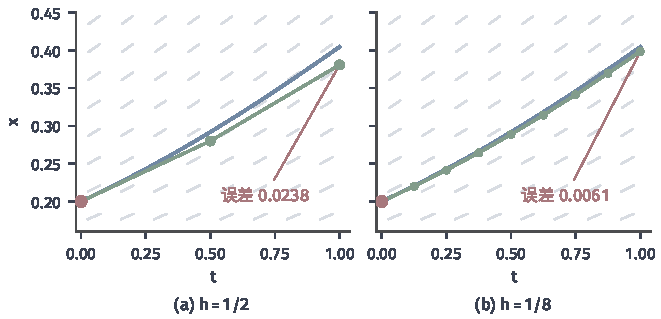
\includegraphics[width=112mm]{figures/06-differential-equations/01-ordinary-differential-equations/matplotlib/odenum-euler-polygon/figure.pdf}
 \caption{显式Euler折线与方向场。灰色短线是$\dot{x}=x(1-x)$的方向场，蓝线为$x(0)=0.2$的真解，绿线和绿点为数值解。(a)$h=1/2$；(b)$h=1/8$。红色标注是$t=1$处的绝对误差。}
 \label{fig:odenum-euler-polygon}
\end{BookInlineFigure}

\paragraph{计算过程}
下面用贯穿全章的初值问题逐步演示，数据为
\begin{equation}
 \dot{x}=x(1-x),\qquad x(0)=0.2,\qquad T=1.
 \label{eq:odenum-running}
\end{equation}
分离变量可得真解，它用来核对数值结果：
\begin{equation}
 x(t)=\frac{1}{1+4\mathrm{e}^{-t}}.
 \label{eq:odenum-running-exact}
\end{equation}
取$h=1/2$，于是$N=2$，手算两步即可走完。

\needspace{6\baselineskip}
\paragraph{变量}
\begin{itemize}
 \item $\bm{x}^{(k)}\in\mathbb{R}^{n}$：第$k$个网格点的数值解。
 \item $t_k$：当前时刻。
 \item $\bm{s}^{(k)}\in\mathbb{R}^{n}$：当前点读到的斜率。
\end{itemize}

\paragraph{初始化}
把数值解初始化为初值，时刻初始化为起点，步长和步数由区间决定：
\[
 \bm{x}^{(0)}=\bm{x}_0,\qquad t_0\text{给定},\qquad h=T/N.
\]
例中
\[
 x^{(0)}=0.2,\qquad t_0=0,\qquad h=0.5,\qquad N=2.
\]

\needspace{6\baselineskip}
\paragraph{每轮更新}
对$k=0,1,\ldots,N-1$依次执行：
\begin{enumerate}
 \item \textbf{读取斜率。}计算
 \[
  \bm{s}^{(k)}=\bm{f}\bigl(t_k,\bm{x}^{(k)}\bigr).
 \]
 例中第一轮
 \[
  s^{(0)}=0.2\times(1-0.2)=0.16.
 \]
 \item \textbf{沿斜率走一步。}由式~\eqref{eq:odenum-euler}计算
 \[
  \bm{x}^{(k+1)}=\bm{x}^{(k)}+h\,\bm{s}^{(k)},\qquad t_{k+1}=t_k+h.
 \]
 例中第一轮
 \[
  x^{(1)}=0.2+0.5\times0.16=0.28,\qquad t_1=0.5.
 \]
 例中第二轮先读斜率，再走一步：
 \[
  s^{(1)}=0.28\times0.72=0.2016,\qquad x^{(2)}=0.28+0.5\times0.2016=0.3808.
 \]
 \item \textbf{停止。}当$k+1=N$时结束。例中$k+1=2$，退出循环。
\end{enumerate}
最终得到网格值$\bm{x}^{(0)},\ldots,\bm{x}^{(N)}$。例中$x^{(2)}=0.3808$，而由式~\eqref{eq:odenum-running-exact}，$x(1)\approx0.404610$，误差约为$-0.0238$。

\paragraph{局部误差}
偏差从何而来？按定义~\ref{def:odenum-errors}，把真解代入一步更新。设$\bm{x}(t)$二次连续可微，含积分余项的Taylor公式给出
\[
 \bm{x}(t_{k+1})=\bm{x}(t_k)+h\dot{\bm{x}}(t_k)+\int_{t_k}^{t_{k+1}}(t_{k+1}-s)\ddot{\bm{x}}(s)\,\mathrm{d}s.
\]
真解满足$\dot{\bm{x}}(t_k)=\bm{f}(t_k,\bm{x}(t_k))$，这一项正好是Euler方法走的那一步，相减后只剩余项。于是显式Euler方法的局部截断误差是
\begin{equation}
 \bm{\ell}^{(k+1)}=-\int_{t_k}^{t_{k+1}}(t_{k+1}-s)\ddot{\bm{x}}(s)\,\mathrm{d}s.
 \label{eq:odenum-euler-local}
\end{equation}
权函数$t_{k+1}-s$在这一步上的积分是$h^2/2$，取范数得到局部误差界
\begin{equation}
 \bigl\lVert\bm{\ell}^{(k+1)}\bigr\rVert_2\leq\frac{h^2}{2}\max_{t\in[t_0,t_0+T]}\bigl\lVert\ddot{\bm{x}}(t)\bigr\rVert_2.
 \label{eq:odenum-euler-local-bound}
\end{equation}

$\ddot{\bm{x}}$由方程自身决定。若$\bm{f}$连续可微，对$\dot{\bm{x}}=\bm{f}(t,\bm{x})$用链式法则，得到
\[
 \ddot{\bm{x}}=\partial_t\bm{f}+\partial_{\bm{x}}\bm{f}\,\bm{f},
\]
右端在$(t,\bm{x}(t))$处取值。$\ddot{\bm{x}}$衡量解曲线弯得多厉害，弯得越厉害，直线走一步偏得越远。

在例~\eqref{eq:odenum-running}中，$\bm{f}$不显含时间，且$\ddot{x}=(1-2x)\dot{x}$。在$t=0$处
\[
 \ddot{x}(0)=(1-0.4)\times0.16=0.096,
\]
所以第一步局部误差的主要部分是$-0.048h^2$。$h=1/2$时它等于$-0.012$，实际的第一步误差是$0.28-0.291875=-0.011875$，两者很接近。图~\ref{fig:odenum-euler-one-step}左侧画出这段偏差，右侧显示步长减半时偏差变为约四分之一。

\begin{BookInlineFigure}
 \centering
 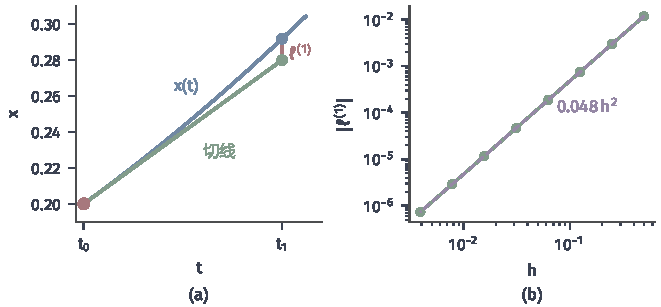
\includegraphics[width=112mm]{figures/06-differential-equations/01-ordinary-differential-equations/matplotlib/odenum-euler-one-step/figure.pdf}
 \caption{显式Euler方法的第一步。(a)$h=1/2$：蓝线是真解，绿线是起点处的切线，红色线段是局部截断误差$\ell^{(1)}$。(b)绿点是不同步长下的$\lvert\ell^{(1)}\rvert$，紫色虚线是主要部分$0.048h^2$。}
 \label{fig:odenum-euler-one-step}
\end{BookInlineFigure}

\begin{definition}[方法的阶]
 \label{def:odenum-order}
 设一步方法的局部截断误差沿真解满足：存在与$k$、$h$无关的$C$和$h_0>0$，使当$0<h\leq h_0$时，对所有$k$有
 \begin{equation}
  \bigl\lVert\bm{\ell}^{(k+1)}\bigr\rVert_2\leq Ch^{p+1},
  \label{eq:odenum-order}
 \end{equation}
 就称方法在这个问题上具有\term{局部误差阶}（local order）$p+1$，称$p$为\term{方法的阶}（order of a method）。
\end{definition}

由式~\eqref{eq:odenum-euler-local-bound}，当$\bm{x}\in C^2$时显式Euler方法的阶为$1$。一步误差$h^2$，方法的阶却是$1$，原因是走完$T$要$N=T/h$步，$N\cdot h^2$恰好是$Th$。这个数步数的算术还不是证明，第~\ref{sec:odenum-error-convergence}节将补全它需要的条件。

\paragraph{步长细化的比较}
一个基本的检验是把步长不断减半，看终点误差怎样变化。表~\ref{tab:odenum-euler-refine}列出例~\eqref{eq:odenum-running}的结果。显式Euler方法每步求值一次右端，所以$N$同时就是计算量。

\begin{BookInlineTable}
 \centering
 \caption{显式Euler方法的步长细化。问题为式~\eqref{eq:odenum-running}，误差指$x^{(N)}-x(1)$，比值是上一行误差除以本行误差。}
 \label{tab:odenum-euler-refine}
 \begin{tabular}{rrrrr}
  \toprule
  $N$ & $h$ & $x^{(N)}$ & 误差 & 比值\\
  \midrule
  2 & 0.5 & 0.380800 & $-2.381\times10^{-2}$ & \\
  4 & 0.25 & 0.392434 & $-1.218\times10^{-2}$ & 1.95\\
  8 & 0.125 & 0.398476 & $-6.134\times10^{-3}$ & 1.99\\
  16 & 0.0625 & 0.401535 & $-3.075\times10^{-3}$ & 1.99\\
  32 & 0.03125 & 0.403071 & $-1.539\times10^{-3}$ & 2.00\\
  \bottomrule
 \end{tabular}
\end{BookInlineTable}

比值趋于$2$：计算量加倍，误差只减半。把误差写成$0.0493/N$（图~\ref{fig:odenum-euler-refinement}），可知要把误差压到$10^{-6}$，约需$5\times10^{4}$次右端求值。对这样一个简单方程，这个价钱是昂贵的，它也给后面的高阶方法提供了比较的基准。

\begin{BookInlineFigure}
 \centering
 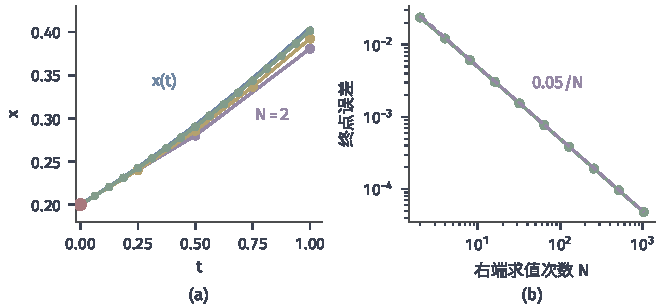
\includegraphics[width=112mm]{figures/06-differential-equations/01-ordinary-differential-equations/matplotlib/odenum-euler-refinement/figure.pdf}
 \caption{显式Euler方法的步长细化。(a)蓝线是真解，紫、黄、绿折线分别是$N=2,4,16$的数值解。(b)$t=1$处的误差随右端求值次数$N$的变化，紫色虚线是参考直线$0.05/N$。}
 \label{fig:odenum-euler-refinement}
\end{BookInlineFigure}


\section{Runge--Kutta方法}
\label{sec:odenum-runge-kutta}

Euler方法整步只用起点的斜率，弯曲的解曲线被它的切线代替。要想更准，自然想到在这一步内部多看几次斜率，再把它们组合起来。看哪几处、怎样组合，才能真正提高阶数？

\paragraph{主要思想：匹配Taylor展开}
先看真解一步走到哪里。设$\bm{f}$二次连续可微，记
\begin{equation}
 \bm{g}=\partial_t\bm{f}+\partial_{\bm{x}}\bm{f}\,\bm{f},
 \label{eq:odenum-total-derivative}
\end{equation}
它是$\bm{f}$沿解的全导数，也就是$\ddot{\bm{x}}$。解的Taylor展开为
\[
 \bm{x}(t+h)=\bm{x}+h\bm{f}+\frac{h^2}{2}\bm{g}+O(h^3),
\]
右端各量在$(t,\bm{x}(t))$处取值。Euler方法只匹配了前两项，$h^2$一项就是它的局部误差。

现在允许多读一次斜率。先取起点斜率，再沿它试探着走到$t+\alpha h$，在那里读第二个斜率：
\[
 \bm{k}_1=\bm{f}(t,\bm{x}),\qquad
 \bm{k}_2=\bm{f}\bigl(t+\alpha h,\bm{x}+\alpha h\bm{k}_1\bigr).
\]
最后用两个斜率的加权平均前进：
\[
 \bm{\Psi}_h(t,\bm{x})=\bm{x}+h\bigl(b_1\bm{k}_1+b_2\bm{k}_2\bigr).
\]

$\alpha,b_1,b_2$待定。把$\bm{k}_2$在$(t,\bm{x})$处作Taylor展开，$h$的一次项正好由式~\eqref{eq:odenum-total-derivative}的全导数给出：
\[
 \bm{k}_2=\bm{f}+\alpha h\,\bm{g}+O(h^2).
\]
代入更新式，得到
\[
 \bm{\Psi}_h(t,\bm{x})=\bm{x}+(b_1+b_2)h\bm{f}+\alpha b_2h^2\bm{g}+O(h^3).
\]

与真解的展开逐项比较，要让$h$和$h^2$的系数都对上，需要
\begin{equation}
 b_1+b_2=1,\qquad \alpha b_2=\frac{1}{2}.
 \label{eq:odenum-two-stage-conditions}
\end{equation}
三个未知数、两个方程，于是有一族二阶方法。取$\alpha=1/2$，$b_1=0$，$b_2=1$，得到\term{中点方法}（midpoint method）：
\begin{equation}
 \begin{aligned}
  \bm{k}_1&=\bm{f}\bigl(t_k,\bm{x}^{(k)}\bigr),\\
  \bm{k}_2&=\bm{f}\Bigl(t_k+\frac{h}{2},\ \bm{x}^{(k)}+\frac{h}{2}\bm{k}_1\Bigr),\\
  \bm{x}^{(k+1)}&=\bm{x}^{(k)}+h\bm{k}_2.
 \end{aligned}
 \label{eq:odenum-midpoint}
\end{equation}
另一个选择$\alpha=1$，$b_1=b_2=1/2$是Heun方法，它在第~\ref{sec:odenum-adaptive}节还要用到。

中点方法的几何含义很清楚（图~\ref{fig:odenum-midpoint-steps}）：积分$\int\bm{f}\,\mathrm{d}s$用区间中点的值乘$h$来近似，这是中点求积公式。困难在于中点处的状态未知，于是先用起点斜率走半步来试探它。试探点本身只有一阶精度，但$\bm{f}$在那里的值只需准到$O(h^2)$，一乘$h$就足够了。

\begin{BookInlineFigure}
 \centering
 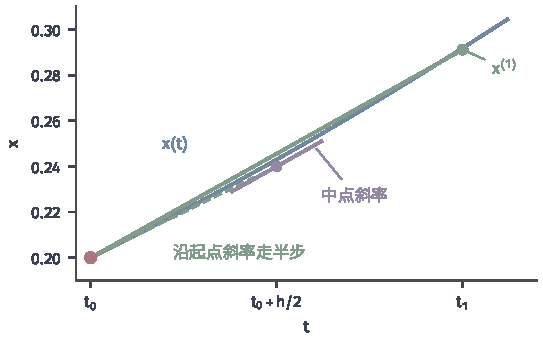
\includegraphics[width=92mm]{figures/06-differential-equations/01-ordinary-differential-equations/matplotlib/odenum-midpoint-steps/figure.pdf}
 \caption{中点方法的第一步，$h=1/2$，问题为式~\eqref{eq:odenum-running}。蓝线是真解，绿色虚线沿起点斜率走半步到紫点，紫色短线是在紫点读到的斜率$k_2$，绿色实线从红色初值出发，沿斜率$k_2$走满一步到$x^{(1)}$。}
 \label{fig:odenum-midpoint-steps}
\end{BookInlineFigure}

中点方法的手算只需把式~\eqref{eq:odenum-midpoint}代入两轮。对例~\eqref{eq:odenum-running}取$h=0.5$，第一轮的结果为
\[
 k_1=0.16,\qquad 0.2+0.25k_1=0.24,\qquad k_2=0.24\times0.76=0.1824,
\]
于是
\[
 x^{(1)}=0.2+0.5\times0.1824=0.2912.
\]
第二轮从$x^{(1)}$出发，同样得到
\[
 k_1=0.206403,\qquad 0.342801,\qquad k_2=0.225288,
\]
所以$x^{(2)}=0.403844$，终点误差约$-7.7\times10^{-4}$，比Euler方法的$-0.0238$小了约三十倍，而右端求值次数只从$2$增加到$4$。

\paragraph{主要思想：多级与经典四阶方法}
上面的做法可以一般化。$s$级\term{显式Runge--Kutta方法}（explicit Runge--Kutta method）依次计算$s$个\term{阶段斜率}（stage slope）：
\begin{equation}
 \bm{k}_i=\bm{f}\Bigl(t_k+c_ih,\ \bm{x}^{(k)}+h\sum_{j<i}a_{i,j}\bm{k}_j\Bigr),\quad i=1,\ldots,s,
 \label{eq:odenum-rk-stages}
\end{equation}
再组合成一步更新：
\begin{equation}
 \bm{x}^{(k+1)}=\bm{x}^{(k)}+h\sum_{i=1}^{s}b_i\bm{k}_i.
 \label{eq:odenum-rk-update}
\end{equation}
每个$\bm{k}_i$只用前面已算出的斜率，所以依次代入即可，这就是“显式”的含义。系数由匹配Taylor展开决定，中点方法是$s=2$的情形。

阶数越高，要匹配的项越多。沿解的高阶全导数含有$\bm{f}$的各阶偏导的多种组合，四阶需要同时满足八个代数条件。最著名的解是\term{经典四阶Runge--Kutta方法}（classical fourth-order Runge--Kutta method），简称RK4：
\begin{equation}
 \begin{aligned}
  \bm{k}_1&=\bm{f}\bigl(t_k,\bm{x}^{(k)}\bigr),\\
  \bm{k}_2&=\bm{f}\Bigl(t_k+\frac{h}{2},\ \bm{x}^{(k)}+\frac{h}{2}\bm{k}_1\Bigr),\\
  \bm{k}_3&=\bm{f}\Bigl(t_k+\frac{h}{2},\ \bm{x}^{(k)}+\frac{h}{2}\bm{k}_2\Bigr),\\
  \bm{k}_4&=\bm{f}\bigl(t_k+h,\ \bm{x}^{(k)}+h\bm{k}_3\bigr),\\
  \bm{x}^{(k+1)}&=\bm{x}^{(k)}+\frac{h}{6}\bigl(\bm{k}_1+2\bm{k}_2+2\bm{k}_3+\bm{k}_4\bigr).
 \end{aligned}
 \label{eq:odenum-rk4}
\end{equation}

权重$1,2,2,1$有一个可以直接验证的来源。若$\bm{f}$不依赖状态，四个斜率分别是$\bm{f}(t_k)$、$\bm{f}(t_k+h/2)$、$\bm{f}(t_k+h/2)$、$\bm{f}(t_k+h)$，更新式化为
\[
 \bm{x}^{(k+1)}-\bm{x}^{(k)}=\frac{h}{6}\Bigl(\bm{f}(t_k)+4\bm{f}\bigl(t_k+\tfrac{h}{2}\bigr)+\bm{f}(t_k+h)\Bigr),
\]
正是Simpson求积公式。中点权重$4$被拆给了两个中点估计$\bm{k}_2$和$\bm{k}_3$，它们从不同的试探点读取斜率，彼此修正。

\begin{theorem}[RK4的阶]
 \label{thm:odenum-rk4-order}
 设$\bm{f}$在包含解曲线的开集上四次连续可微，$\bm{x}(t)$是$[t_0,t_0+T]$上的解。则存在$C,h_0>0$，使当$0<h\leq h_0$时，RK4的局部截断误差满足
 \begin{equation}
  \bigl\lVert\bm{\ell}^{(k+1)}\bigr\rVert_2\leq Ch^{5}.
  \label{eq:odenum-rk4-local}
 \end{equation}
\end{theorem}

这个结论的证明需要把真解和数值更新都展开到$h^4$，逐项核对八个代数条件，篇幅较长，读者可查阅\scite{math-hairer1993ode}。定理的条件不能省：光滑性决定了展开能够进行到第几项，下文的例子会说明它不成立时阶数怎样丢失。

\paragraph{计算过程}
RK4每一步按式~\eqref{eq:odenum-rk4}依次算四个斜率。下面仍用例~\eqref{eq:odenum-running}的数据手算，取$h=0.5$，$N=2$。

\needspace{6\baselineskip}
\paragraph{变量}
\begin{itemize}
 \item $\bm{x}^{(k)}\in\mathbb{R}^{n}$：第$k$个网格点的数值解。
 \item $\bm{k}_1,\bm{k}_2,\bm{k}_3,\bm{k}_4\in\mathbb{R}^{n}$：本步的四个阶段斜率，用完即弃。
 \item $\bm{y}_2,\bm{y}_3,\bm{y}_4\in\mathbb{R}^{n}$：读取后三个斜率的试探状态。
\end{itemize}

\paragraph{初始化}
与Euler方法相同，把数值解初始化为初值。例中
\[
 x^{(0)}=0.2,\qquad t_0=0,\qquad h=0.5,\qquad N=2.
\]

\needspace{6\baselineskip}
\paragraph{每轮更新}
对$k=0,1,\ldots,N-1$依次执行：
\begin{enumerate}

 \item \textbf{起点斜率。}计算$\bm{k}_1=\bm{f}(t_k,\bm{x}^{(k)})$。例中第一轮
 \[
  k_1=0.2\times0.8=0.16.
 \]

 \item \textbf{第一次试探中点。}令
 \[
  \bm{y}_2=\bm{x}^{(k)}+\frac{h}{2}\bm{k}_1,\qquad \bm{k}_2=\bm{f}\bigl(t_k+\tfrac{h}{2},\bm{y}_2\bigr).
 \]
 例中第一轮
 \[
  y_2=0.24,\qquad k_2=0.24\times0.76=0.1824.
 \]

 \item \textbf{第二次试探中点。}令
 \[
  \bm{y}_3=\bm{x}^{(k)}+\frac{h}{2}\bm{k}_2,\qquad \bm{k}_3=\bm{f}\bigl(t_k+\tfrac{h}{2},\bm{y}_3\bigr).
 \]
 例中第一轮
 \[
  y_3=0.2456,\qquad k_3=0.2456\times0.7544=0.185281.
 \]

 \item \textbf{试探终点。}令
 \[
  \bm{y}_4=\bm{x}^{(k)}+h\bm{k}_3,\qquad \bm{k}_4=\bm{f}\bigl(t_k+h,\bm{y}_4\bigr).
 \]
 例中第一轮
 \[
  y_4=0.292640,\qquad k_4=0.207002.
 \]

 \item \textbf{加权前进。}由式~\eqref{eq:odenum-rk4}的最后一行计算$\bm{x}^{(k+1)}$。例中第一轮
 \[
  x^{(1)}=0.2+\frac{0.5}{6}\times1.102363=0.2918636.
 \]
 例中第二轮从$x^{(1)}$出发，依次得到
 \[
  \begin{gathered}
   k_1=0.206679,\quad y_2=0.343533,\quad k_2=0.225518,\\
   y_3=0.348243,\quad k_3=0.226970,\\
   y_4=0.405349,\quad k_4=0.241041,
  \end{gathered}
 \]
 于是
 \[
  x^{(2)}=0.2918636+\frac{0.5}{6}\times1.352696=0.4045883.
 \]

 \item \textbf{停止。}当$k+1=N$时结束。例中$k+1=2$，退出循环。
\end{enumerate}
最终例中得到$x^{(2)}=0.404588$，真值为$0.404610$，误差约$-2.1\times10^{-5}$，只用了$8$次右端求值。图~\ref{fig:odenum-rk4-stages}标出第一步的四个采样位置。

\begin{BookInlineFigure}
 \centering
 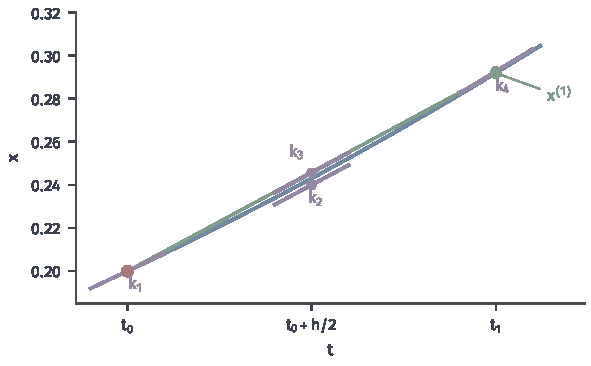
\includegraphics[width=100mm]{figures/06-differential-equations/01-ordinary-differential-equations/matplotlib/odenum-rk4-stages/figure.pdf}
 \caption{RK4的第一步，$h=1/2$，问题为式~\eqref{eq:odenum-running}。紫点是四个采样位置$(t_0,x_0)$、$(t_0+h/2,y_2)$、$(t_0+h/2,y_3)$、$(t_1,y_4)$，紫色短线是读到的四个斜率；绿线从红色初值走到$x^{(1)}$，蓝线是真解。}
 \label{fig:odenum-rk4-stages}
\end{BookInlineFigure}

\paragraph{光滑性决定阶数能否兑现}
定理~\ref{thm:odenum-rk4-order}要求右端足够光滑。把例~\eqref{eq:odenum-running}改成带时间跳变的方程：
\[
 \dot{x}=r(t)x(1-x),\qquad
 r(t)=\begin{cases}1,&t<t_{*},\\2,&t\geq t_{*},\end{cases}
\]
其中$t_{*}=1/\sqrt{2}$，闭式解用$\int_0^tr$代替$t$仍然成立。图~\ref{fig:odenum-rk4-jump}的红线是均匀网格上RK4的终点误差。$t_{*}$落在某一步内部，四个采样点无法判断跳变发生在这一步的什么位置，这一步的局部误差只有$O(h)$，一步就把全局误差拖到一阶，并随$t_{*}$在步内的相对位置起伏。

\begin{BookInlineFigure}
 \centering
 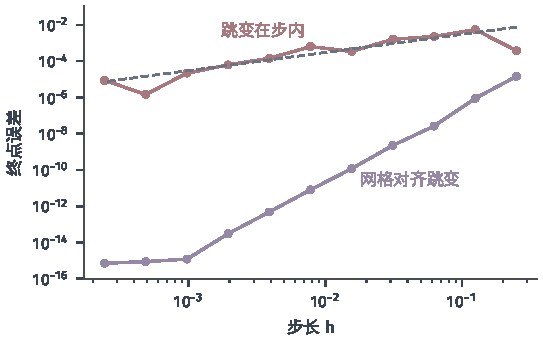
\includegraphics[width=92mm]{figures/06-differential-equations/01-ordinary-differential-equations/matplotlib/odenum-rk4-jump/figure.pdf}
 \caption{右端带跳变时RK4的终点误差。红线：均匀网格，跳变点$t_{*}=1/\sqrt{2}$落在步内；灰色虚线是参考直线$0.03h$。紫线：把$t_{*}$放在网格点上，两侧分别用均匀步长积分，四阶恢复，直到舍入误差使曲线变平。}
 \label{fig:odenum-rk4-jump}
\end{BookInlineFigure}

补救办法也在图中。若已知跳变时刻，把它放到网格点上，在两侧分别积分（紫线），每段内部$\bm{f}$都是光滑的，阶数恢复为四。

\paragraph{每步成本与总成本}
高阶方法每步更贵，比较时必须看走完全程的总求值次数。图~\ref{fig:odenum-rk-convergence}左图的三条直线斜率分别为$1$、$2$、$4$，与三个方法的阶一致。右图把横轴换成右端求值次数，表~\ref{tab:odenum-cost}给出达到同一精度的成本。

\begin{BookInlineFigure}
 \centering
 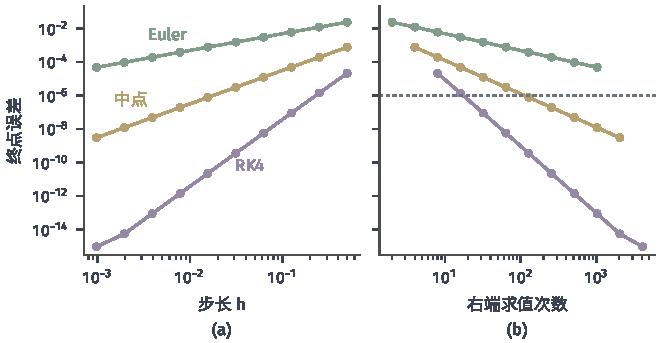
\includegraphics[width=112mm]{figures/06-differential-equations/01-ordinary-differential-equations/matplotlib/odenum-rk-convergence/figure.pdf}
 \caption{三种方法在式~\eqref{eq:odenum-running}上$t=1$处的误差。绿、黄、紫线分别是Euler、中点、RK4。(a)误差对步长；(b)误差对右端求值次数，灰色虚线是$10^{-6}$。RK4在$h$很小时误差碰到舍入水平。}
 \label{fig:odenum-rk-convergence}
\end{BookInlineFigure}

\begin{BookInlineTable}
 \centering
 \caption{式~\eqref{eq:odenum-running}上使$t=1$处误差不超过给定精度所需的右端求值次数（步数以约$3\%$递增搜索，故为近似值）。}
 \label{tab:odenum-cost}
 \begin{tabular}{rrrr}
  \toprule
  目标精度 & Euler（每步1次） & 中点（每步2次） & RK4（每步4次）\\
  \midrule
  $10^{-2}$ & 5 & 2 & 4\\
  $10^{-4}$ & $5.0\times10^{2}$ & 12 & 8\\
  $10^{-6}$ & $4.9\times10^{4}$ & $1.2\times10^{2}$ & 20\\
  $10^{-8}$ & $5.0\times10^{6}$ & $1.1\times10^{3}$ & 56\\
  \bottomrule
 \end{tabular}
\end{BookInlineTable}

表中的规律是：精度要求越高，高阶方法的优势越大；要求只有$10^{-2}$时，三者的成本差不多，RK4反而比中点方法多花一倍。这个比较只在解足够光滑时有意义，图~\ref{fig:odenum-rk4-jump}的情形下RK4多花的求值次数并不能换来四阶精度。



\section{误差与收敛}
\label{sec:odenum-error-convergence}

前两节看到的现象是：一步误差为$h^{p+1}$时，终点误差表现为$h^{p}$。数步数的算术说明不了这件事，因为早期产生的误差还要被后面的每一步继续传播，可能被放大。什么条件下这种累积可控？

\paragraph{一步局部误差的约定}
先把量纲说清楚。本书的局部截断误差~\eqref{eq:odenum-local-error}没有除以步长，它是一步之内产生的偏差，单位与状态相同。若方法的阶为$p$，它的大小是$O(h^{p+1})$。

有些文献把$\bm{\ell}^{(k+1)}/h$称为截断误差，这时阶为$p$的方法“局部截断误差”写作$O(h^{p})$。两种写法描述同一件事，读其他资料时要先确认定义。下表对比本章会用到的两个量。

\begin{BookInlineTable}
 \centering
 \caption{局部截断误差与全局误差的对比（阶为$p$的方法）。}
 \label{tab:odenum-local-global}
 \begin{tabular}{lll}
  \toprule
  & 局部截断误差$\bm{\ell}^{(k+1)}$ & 全局误差$\bm{e}^{(k)}$\\
  \midrule
  出发点 & 真解点$\bm{x}(t_k)$ & 实际算出的序列\\
  包含 & 一步更新的缺陷 & 全部历史的累积\\
  大小 & $O(h^{p+1})$ & 条件满足时$O(h^{p})$\\
  能否实际算出 & 需要真解 & 需要真解\\
  \bottomrule
 \end{tabular}
\end{BookInlineTable}

\paragraph{误差的传播图景}
式~\eqref{eq:odenum-error-split}说明每步的新误差与旧误差叠加。还可以换一个角度看：每步产生的偏差会被此后的真实流映射搬运到终点。把$\bm{\varphi}_{t,t_N}$作用于网格值，相邻两项之差就是第$k$步的贡献，它们相加后中间项全部抵消，在没有初值误差时得到
\begin{equation}
 \bm{e}^{(N)}=\sum_{k=0}^{N-1}\Bigl[\bm{\varphi}_{t_{k+1},t_N}\bigl(\bm{x}^{(k+1)}\bigr)-\bm{\varphi}_{t_k,t_N}\bigl(\bm{x}^{(k)}\bigr)\Bigr].
 \label{eq:odenum-telescoping}
\end{equation}

图~\ref{fig:odenum-error-fan}左侧画出这个分解。绿色折线是Euler网格值与真解之差，每个绿点处长出一条黄线，它是从该点出发的真解。相邻黄线在终点的间距，正是式~\eqref{eq:odenum-telescoping}的一项。

\begin{BookInlineFigure}
 \centering
 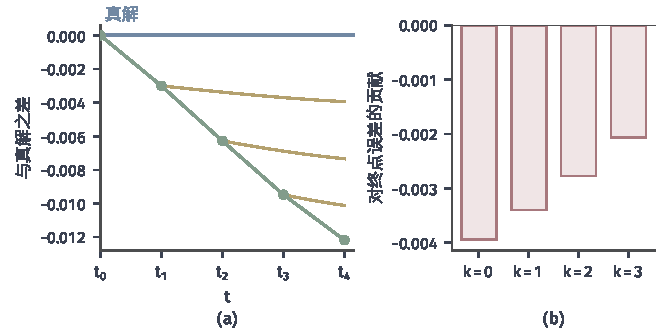
\includegraphics[width=112mm]{figures/06-differential-equations/01-ordinary-differential-equations/matplotlib/odenum-error-fan/figure.pdf}
 \caption{显式Euler方法的误差累积，问题为式~\eqref{eq:odenum-running}，$h=1/4$。(a)纵轴是与真解之差：蓝线是真解，绿线是网格值，黄线是从各网格值出发的真解。(b)式~\eqref{eq:odenum-telescoping}的四项，即每步偏差被搬运到$t=1$时的大小，四项之和等于终点误差$-0.01218$。}
 \label{fig:odenum-error-fan}
\end{BookInlineFigure}

例中四项依次为$-0.00394$、$-0.00340$、$-0.00277$、$-0.00206$，第一步的贡献最大。第一步本身的局部误差只有$-0.00300$，搬运到终点后变成$-0.00394$，因为这里$\partial_xf=1-2x>0$，邻近的解随时间分开。流映射放大扰动的程度决定了累积的结果，这与第~\ref{chap:ode-sensitivity}章的结论是同一回事。

\paragraph{一步稳定性}
要给出误差界，需要一个条件控制式~\eqref{eq:odenum-error-split}的第一项。连续情形的对应结论是Gronwall估计：若$\bm{f}$关于状态满足Lipschitz条件，常数为$L$，则从两个初值出发的解之差至多按$\mathrm{e}^{L(t-s)}$增长，推导见第~\ref{chap:ode-sensitivity}章。离散情形要求的是这种增长的一步版本。

数值解只需要在真解附近受控。取半径$\rho>0$，记真解周围的管状区域为
\begin{equation}
 \bm{K}_{\rho}=\bigl\{(t,\bm{y}):t\in[t_0,t_0+T],\ \lVert\bm{y}-\bm{x}(t)\rVert_2\leq\rho\bigr\}.
 \label{eq:odenum-tube}
\end{equation}

\begin{definition}[一步稳定性]
 \label{def:odenum-one-step-stability}
 设存在$\Lambda>0$和$h_0>0$，使当$0<h\leq h_0$时，对$\bm{K}_{\rho}$中所有同一时刻$t$的点$(t,\bm{y})$与$(t,\bm{z})$都有
 \begin{equation}
  \bigl\lVert\bm{\Psi}_h(t,\bm{y})-\bm{\Psi}_h(t,\bm{z})\bigr\rVert_2\leq(1+h\Lambda)\lVert\bm{y}-\bm{z}\rVert_2,
  \label{eq:odenum-one-step-stability}
 \end{equation}
 就称一步方法在$\bm{K}_{\rho}$上具有\term{一步稳定性}（one-step stability）。
\end{definition}

式中放大因子写成$1+h\Lambda$有明确的用意。走$N=T/h$步，累积因子至多是$(1+h\Lambda)^{T/h}\leq\mathrm{e}^{\Lambda T}$，不随$h\to0$增大。如果放大因子只是$1+\sqrt{h}$，下文会看到累积因子将趋于无穷。

这个条件可以逐个方法验证。设$\bm{f}$关于状态的Lipschitz常数在所考虑的区域上为$L$。显式Euler方法两点的差是
\[
 \bigl\lVert\bm{\Psi}_h(t,\bm{y})-\bm{\Psi}_h(t,\bm{z})\bigr\rVert_2
 \leq\lVert\bm{y}-\bm{z}\rVert_2+h\bigl\lVert\bm{f}(t,\bm{y})-\bm{f}(t,\bm{z})\bigr\rVert_2,
\]
第二项不超过$hL\lVert\bm{y}-\bm{z}\rVert_2$，所以$\Lambda=L$。

中点方法要多一层试探点。设$\bm{f}$在更大的管$\bm{K}_{2\rho}$上有界、Lipschitz常数为$L$，$h_0$足够小，使试探点仍在$\bm{K}_{2\rho}$内。两个点的第一个斜率之差不超过$L\lVert\bm{y}-\bm{z}\rVert_2$，第二个斜率之差满足
\[
 \lVert\bm{k}_2-\bm{k}_2'\rVert_2\leq L\Bigl(1+\frac{hL}{2}\Bigr)\lVert\bm{y}-\bm{z}\rVert_2.
\]
于是中点方法满足式~\eqref{eq:odenum-one-step-stability}，常数为
\[
 \Lambda=L\Bigl(1+\frac{h_0L}{2}\Bigr).
\]

一般的显式Runge--Kutta方法做法相同。由式~\eqref{eq:odenum-rk-stages}逐级得到
\[
 \lVert\bm{k}_i-\bm{k}_i'\rVert_2\leq L\Bigl(\lVert\bm{y}-\bm{z}\rVert_2+h\sum_{j<i}\lvert a_{i,j}\rvert\,\lVert\bm{k}_j-\bm{k}_j'\rVert_2\Bigr),
\]
级数有限，归纳即可得到形如式~\eqref{eq:odenum-one-step-stability}的估计，$\Lambda$由$L$、系数和$h_0$决定。

\paragraph{离散Gronwall不等式}
把一步稳定性代入式~\eqref{eq:odenum-error-split}，会得到一个数列的递推不等式。下面的引理把这种递推解开，它是连续Gronwall估计的离散版本。

\begin{lemma}[离散Gronwall不等式]
 \label{lem:odenum-discrete-gronwall}
 设$q>0$，$b\geq0$，非负数列满足$a_{j+1}\leq(1+q)a_j+b$，$j=0,\ldots,m-1$。则对$j=0,\ldots,m$，
 \begin{equation}
  a_j\leq(1+q)^{j}a_0+\frac{(1+q)^{j}-1}{q}\,b.
  \label{eq:odenum-discrete-gronwall}
 \end{equation}
\end{lemma}

\begin{proof}
 对$j$作归纳。$j=0$时不等式两边都是$a_0$。

 设式~\eqref{eq:odenum-discrete-gronwall}对$j$成立，把它代入$a_{j+1}\leq(1+q)a_j+b$，得到
 \[
  a_{j+1}\leq(1+q)^{j+1}a_0+\Bigl[(1+q)\frac{(1+q)^{j}-1}{q}+1\Bigr]b.
 \]
 通分后方括号内的量化简为
 \[
  \frac{(1+q)^{j+1}-(1+q)+q}{q}=\frac{(1+q)^{j+1}-1}{q},
 \]
 这正是$j+1$时的结论。
\end{proof}

\paragraph{全局误差定理}
现在把三种误差放到一起。

\begin{theorem}[有限区间上的全局误差界]
 \label{thm:odenum-global-error}
 设$\bm{x}(t)$是式~\eqref{eq:odenum-ivp}在$[t_0,t_0+T]$上的解，一步方法在$\bm{K}_{\rho}$上满足一步稳定性~\eqref{eq:odenum-one-step-stability}，并且对$0<h\leq h_0$与所有$k$，
 \begin{equation}
  \bigl\lVert\bm{\ell}^{(k+1)}\bigr\rVert_2\leq Ch^{p+1},\quad
  \bigl\lVert\bm{\delta}^{(0)}\bigr\rVert_2\leq\varepsilon_0,\quad
  \bigl\lVert\bm{\delta}^{(k+1)}\bigr\rVert_2\leq\varepsilon.
  \label{eq:odenum-global-hypotheses}
 \end{equation}
 记
 \begin{equation}
  E(h)=\mathrm{e}^{\Lambda T}\varepsilon_0+\frac{\mathrm{e}^{\Lambda T}-1}{\Lambda}\Bigl(Ch^{p}+\frac{\varepsilon}{h}\Bigr).
  \label{eq:odenum-global-bound-def}
 \end{equation}
 若$h\leq h_0$且$E(h)\leq\rho$，则式~\eqref{eq:odenum-computed}的序列都留在管内，并且对$k=0,1,\ldots,N$，
 \begin{equation}
  \bigl\lVert\bm{e}^{(k)}\bigr\rVert_2\leq\mathrm{e}^{\Lambda kh}\varepsilon_0+\frac{\mathrm{e}^{\Lambda kh}-1}{\Lambda}\Bigl(Ch^{p}+\frac{\varepsilon}{h}\Bigr)\leq E(h).
  \label{eq:odenum-global-bound}
 \end{equation}
\end{theorem}

\begin{proof}
 记$a_k=\lVert\bm{e}^{(k)}\rVert_2$，$q=h\Lambda$，$b=Ch^{p+1}+\varepsilon$。对$k$归纳证明式~\eqref{eq:odenum-global-bound}，同时得到$(t_k,\bm{x}^{(k)})\in\bm{K}_{\rho}$。

 $k=0$时$a_0\leq\varepsilon_0\leq E(h)\leq\rho$。

 设直到$k$结论都成立，那么$\bm{x}^{(k)}$与$\bm{x}(t_k)$都在管内，可以对式~\eqref{eq:odenum-error-split}用一步稳定性和假设~\eqref{eq:odenum-global-hypotheses}，得到
 \[
  a_{j+1}\leq(1+q)a_j+b,\qquad j=0,\ldots,k.
 \]
 由引理~\ref{lem:odenum-discrete-gronwall}，
 \[
  a_{k+1}\leq(1+q)^{k+1}a_0+\frac{(1+q)^{k+1}-1}{q}\,b.
 \]

 用$1+q\leq\mathrm{e}^{q}$，且$q=h\Lambda$，第一项不超过$\mathrm{e}^{\Lambda(k+1)h}\varepsilon_0$。第二项的系数满足
 \[
  \frac{(1+q)^{k+1}-1}{q}\,b\leq\frac{\mathrm{e}^{\Lambda(k+1)h}-1}{h\Lambda}\,b.
 \]
 其中$b/h=Ch^{p}+\varepsilon/h$，所以式~\eqref{eq:odenum-global-bound}对$k+1$成立。

 因为$(k+1)h\leq T$，右端不超过$E(h)\leq\rho$，$\bm{x}^{(k+1)}$仍在管内，归纳完成。
\end{proof}

式~\eqref{eq:odenum-global-bound}的三项对应三种误差。初值误差被放大$\mathrm{e}^{\Lambda T}$倍。截断误差每步$Ch^{p+1}$，共$T/h$步，累积成$Ch^{p}$的量级，常数$(\mathrm{e}^{\Lambda T}-1)/\Lambda$扮演放大因子。计算误差同样累积，但少除了一次$h$，留下$\varepsilon/h$。

\paragraph{算例：误差界与实际误差}
\begin{example}[Euler方法的误差界]
 \label{ex:odenum-euler-bound}
 对例~\eqref{eq:odenum-running}用显式Euler方法，并设计算无误差。

 取$\rho=0.1$。真解在$[0,1]$上取值于$[0.2,0.4047]$，所以管内状态落在$[0.1,0.505]$中，在这里
 \[
  \lvert\partial_xf\rvert=\lvert1-2x\rvert\leq0.8,
 \]
 可取$\Lambda=L=0.8$。

 由$\ddot{x}=(1-2x)x(1-x)$，它在$[0.2,0.4047]$上的最大值约为$0.0962$，在$x\approx0.2113$处取得。由式~\eqref{eq:odenum-euler-local-bound}可取
 \[
  C=\frac{0.0962}{2}=0.0481,\qquad p=1.
 \]

 代入式~\eqref{eq:odenum-global-bound-def}，$\varepsilon_0=\varepsilon=0$，得到
 \[
  E(h)=\frac{\mathrm{e}^{0.8}-1}{0.8}\times0.0481\,h\approx0.0737\,h.
 \]
 $h=0.5$时$E(h)\approx0.0368$，满足$E(h)\leq\rho$，实际误差$0.0238$在这个界内。当$h\to0$时实际误差约为$0.0493h$，界比它大约百分之五十。
\end{example}

\paragraph{一步误差的阶何时给出全局误差的阶}
定理~\ref{thm:odenum-global-error}给出了答案。取$\varepsilon_0=O(h^{p})$，$\varepsilon=O(h^{p+1})$，又要$\bm{\ell}^{(k+1)}=O(h^{p+1})$在所有步上一致成立，方法一步稳定，并且真解在整个区间存在，那么全局误差就是$O(h^{p})$。下面逐条看去掉条件会怎样。

\emph{没有一步稳定性。}考虑$\dot{x}=0$，$x(0)=0$，真解恒为零，取映射
\[
 \Psi_h(y)=(1+\sqrt{h})\,y.
\]
沿真解$\Psi_h(0)=0$，局部截断误差严格为零。可是放大因子是$1+\sqrt{h}$，不是$1+O(h)$。给初值一个$h^2$的扰动，走到$T=1$后得到
\[
 \lvert x^{(N)}\rvert=(1+\sqrt{h})^{1/h}h^{2}.
\]
$h=0.01$时它约等于$1.38$，并且$h\to0$时趋于无穷。局部误差再小也不能保证收敛。

\emph{局部误差只在部分步上达到高阶。}图~\ref{fig:odenum-rk4-jump}就是这种情形：跳变所在的那一步局部误差只有$O(h)$，其余各步是$O(h^{5})$，全局误差被那一步决定，退回一阶。

\emph{初值误差和计算误差不随步长减小。}固定的$\varepsilon_0$只给出误差的下限。更值得注意的是计算误差项$\varepsilon/h$：它随$h$减小而增大，于是全局误差关于步长是一个先降后升的曲线。对$Ch^{p}+\varepsilon/h$求最小，当$p=1$时
\[
 h_{*}=\sqrt{\frac{\varepsilon}{C}},
\]
此时最小值为$2\sqrt{C\varepsilon}$。图~\ref{fig:odenum-roundoff-v}把Euler方法每步的结果舍入到小数点后六位，亲手制造了这个现象。

\begin{BookInlineFigure}
 \centering
 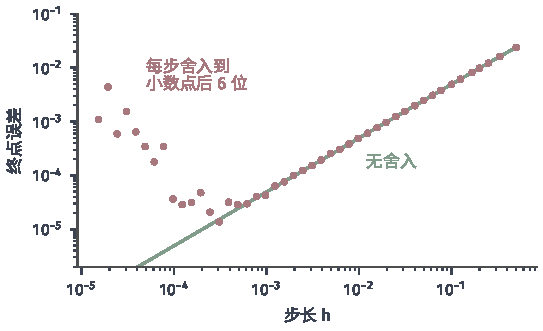
\includegraphics[width=92mm]{figures/06-differential-equations/01-ordinary-differential-equations/matplotlib/odenum-roundoff-v/figure.pdf}
 \caption{显式Euler方法的截断误差与舍入误差，问题为式~\eqref{eq:odenum-running}，$T=1$。绿线不作舍入，红点是每步把结果舍入到小数点后六位时的终点误差。$h$太大时截断误差主导，$h$太小时舍入误差累积主导。}
 \label{fig:odenum-roundoff-v}
\end{BookInlineFigure}

图中误差的最小值约为$10^{-5}$，出现在$h\approx3\times10^{-4}$附近，再缩小步长，误差反而变大。这比最坏情形的界算出的$h_{*}$更小，因为实际舍入有正有负、部分抵消，定理~\ref{thm:odenum-global-error}只给出上界。

\emph{真解在区间上不存在。}对$\dot{x}=x^2$，$x(0)=1$，解在$t=1$爆炸，定理的条件不成立。Euler方法却照常输出，取$h=0.5$走到$t=2$：
\[
 1,\quad 1.5,\quad 2.625,\quad 6.070,\quad 24.495.
\]
数值方法给出有限的数字，并不说明解在那里存在，第~\ref{chap:ode-existence-continuation}章的延拓判据不能省。


\section{刚性问题}
\label{sec:odenum-stiff}

到目前为止，步长的选择只由精度决定。可是有一类方程，解已经很平缓了，显式方法仍然被迫走极小的步，否则数值解会炸开。先看一个具体的系统。

\paragraph{快速分量追随缓慢分量}
设$x_1$按单位速率衰减，$x_2$以很快的速率追随$x_1$：
\begin{equation}
 \dot{x}_1=-x_1,\qquad \dot{x}_2=50(x_1-x_2),\qquad \bm{x}(0)=\begin{bmatrix}1\\0\end{bmatrix}.
 \label{eq:odenum-stiff-system}
\end{equation}
写成矩阵形式，$\dot{\bm{x}}=\bm{A}\bm{x}$，系数矩阵的特征值是$-1$和$-50$：
\[
 \bm{A}=\begin{bmatrix}-1&0\\50&-50\end{bmatrix}.
\]
线性方程的解法见第~\ref{chap:linear-differential-systems}章，这里直接解出真解：
\begin{equation}
 x_1(t)=\mathrm{e}^{-t},\qquad x_2(t)=\frac{50}{49}\bigl(\mathrm{e}^{-t}-\mathrm{e}^{-50t}\bigr).
 \label{eq:odenum-stiff-exact}
\end{equation}

$\mathrm{e}^{-50t}$一项在$t=0.1$时已经小于$0.7\%$，此后解几乎就是缓慢的$\mathrm{e}^{-t}$（图~\ref{fig:odenum-stiff-scales}）。要描绘这条平缓曲线，步长取$0.1$左右就够了，因为此后真解的时间尺度是$1$。

\begin{BookInlineFigure}
 \centering
 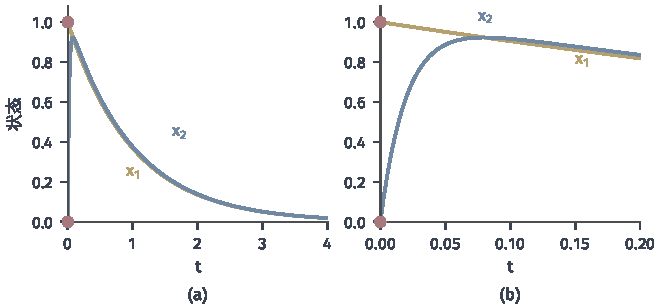
\includegraphics[width=112mm]{figures/06-differential-equations/01-ordinary-differential-equations/matplotlib/odenum-stiff-scales/figure.pdf}
 \caption{系统~\eqref{eq:odenum-stiff-system}的真解，蓝线为$x_2$，黄线为$x_1$，红点是初值。(a)整个区间，两条曲线在初始瞬间之后几乎重合。(b)放大开头的$t\in[0,0.2]$：$x_2$在大约$0.1$的时间内快速追上$x_1$。}
 \label{fig:odenum-stiff-scales}
\end{BookInlineFigure}

\paragraph{显式方法的步长限制}
对这个系统用显式Euler方法。$x_2$的更新是
\[
 x_2^{(k+1)}=(1-50h)\,x_2^{(k)}+50h\,x_1^{(k)}.
\]
括号里的$1-50h$是$x_2$的偏差每步被乘上的因子。$\lvert1-50h\rvert>1$时，偏差逐步放大，真解的平缓与否都救不了它。

取$h=0.05$，因子是$-1.5$，$x_2$的前几步是
\[
 2.5,\quad -1.375,\quad 4.319,\quad -4.335,
\]
而真解在$0.83$到$0.92$之间。取$h=0.03$，因子是$-0.5$，前几步是
\[
 1.5,\quad 0.705,\quad 1.059,\quad 0.840,
\]
逐渐稳定到真解附近（图~\ref{fig:odenum-stiff-euler}）。

\begin{BookInlineFigure}
 \centering
 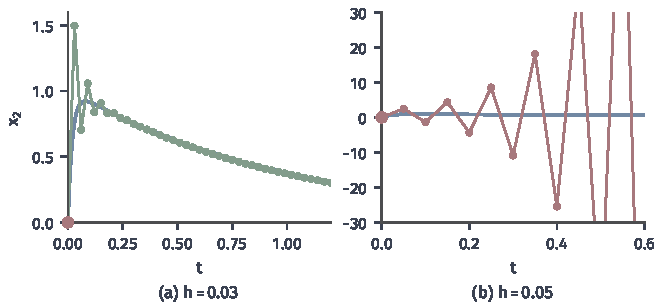
\includegraphics[width=112mm]{figures/06-differential-equations/01-ordinary-differential-equations/matplotlib/odenum-stiff-euler/figure.pdf}
 \caption{显式Euler方法用于系统~\eqref{eq:odenum-stiff-system}的$x_2$分量。蓝线是真解，红点是初值，折线是数值解。(a)$h=0.03$，一步因子$-0.5$，振荡衰减，绿线贴回真解。(b)$h=0.05$，一步因子$-1.5$，红线每步变号并放大。注意两图纵轴的范围不同。}
 \label{fig:odenum-stiff-euler}
\end{BookInlineFigure}

分界在$h=2/50=0.04$。这个限制来自早已衰减殆尽的快速分量，而不是来自要描绘的慢曲线。若把快速率从$50$提高到$5000$，步长上限就成了$4\times10^{-4}$，真解的慢曲线却没有任何变化。

像这样，稳定性对步长的要求比精度的要求严格得多的问题，称为\term{刚性问题}（stiff problem）。刚性没有一个公认的严格定义，它描述的是方程、方法和精度目标三者之间的关系：同一个方程，若目标就是精确刻画开头的快速过程，小步长是精度本身的需要，那就算不上刚性带来的麻烦。

第~\ref{sec:odenum-error-convergence}节的误差界在这里帮不上忙。系统的Lipschitz常数大约是$50$，定理~\ref{thm:odenum-global-error}的放大因子$\mathrm{e}^{\Lambda T}$在$T=4$时是$\mathrm{e}^{200}$量级。Lipschitz常数只看变化率的大小，看不出快速模式是在衰减还是在增长，所以需要另一种分析。

\subsection{绝对稳定性}
\label{sec:odenum-absolute-stability}

固定步长$h$，让步数不断增加，数值解中的扰动是衰减还是放大？回答这个问题的标准工具是一个最简单的方程。

\paragraph{测试方程与放大因子}
取标量线性方程，$\lambda$允许为复数，复数$\lambda$对应振荡的模式：
\begin{equation}
 \dot{x}=\lambda x,\qquad \lambda\in\mathbb{C}.
 \label{eq:odenum-test-equation}
\end{equation}
它称为\term{测试方程}（test equation）。对这个方程，一步方法每步把数值解乘上一个只依赖$z=h\lambda$的数$R(z)$，$R$称为方法的\term{放大因子}（amplification factor），也叫稳定函数。

逐个方法代入。显式Euler方法给出
\[
 x^{(k+1)}=x^{(k)}+h\lambda x^{(k)},
\]
所以$R(z)=1+z$。

中点方法的两个斜率分别是
\[
 k_1=\lambda x^{(k)},\qquad k_2=\lambda\Bigl(1+\frac{z}{2}\Bigr)x^{(k)},
\]
代入更新式$x^{(k+1)}=x^{(k)}+hk_2$，得到
\[
 R(z)=1+z+\frac{z^2}{2}.
\]

RK4的四个斜率依次为
\[
 \begin{aligned}
  k_1&=\lambda x^{(k)},\\
  k_2&=\lambda\Bigl(1+\frac{z}{2}\Bigr)x^{(k)},\\
  k_3&=\lambda\Bigl(1+\frac{z}{2}+\frac{z^2}{4}\Bigr)x^{(k)},\\
  k_4&=\lambda\Bigl(1+z+\frac{z^2}{2}+\frac{z^3}{4}\Bigr)x^{(k)}.
 \end{aligned}
\]
代入$\tfrac{h}{6}(k_1+2k_2+2k_3+k_4)$并合并同类项，得到
\[
 R(z)=1+z+\frac{z^2}{2}+\frac{z^3}{6}+\frac{z^4}{24}.
\]

三个放大因子都是$\mathrm{e}^{z}$的Taylor截断，截断的次数恰好等于方法的阶。真解每步被乘$\mathrm{e}^{z}$，$R(z)$就是对它的近似。

\begin{definition}[绝对稳定域]
 \label{def:odenum-stability-region}
 一步方法用于测试方程~\eqref{eq:odenum-test-equation}时若满足$x^{(k+1)}=R(z)x^{(k)}$，称
 \begin{equation}
  \bm{S}=\bigl\{z\in\mathbb{C}:\lvert R(z)\rvert\leq1\bigr\}
  \label{eq:odenum-stability-region}
 \end{equation}
 为方法的\term{绝对稳定域}（region of absolute stability）。
\end{definition}

当$\mathrm{Re}\,\lambda<0$时，测试方程的真解衰减，$\lvert\mathrm{e}^{z}\rvert<1$。我们希望数值解也不放大，这就要求$h\lambda$落在稳定域内。

\paragraph{从测试方程到线性系统}
为什么一个标量方程能说明系统的问题？设$\bm{A}$可对角化，$\bm{A}=\bm{V}\bm{D}\bm{V}^{-1}$。令$\bm{w}=\bm{V}^{-1}\bm{x}$，对显式Euler方法，
\[
 \bm{w}^{(k+1)}=(\bm{I}+h\bm{D})\bm{w}^{(k)},
\]
每个模式各自按测试方程演化。其他Runge--Kutta方法同样如此，因为它们都只用$\bm{A}$的多项式。

于是数值解不放大的条件是每个$h\lambda_i$都落在$\bm{S}$中。对系统~\eqref{eq:odenum-stiff-system}，$\lambda=-1$给出$z=-h$，$\lambda=-50$给出$z=-50h$；后者的约束才是起作用的。

\paragraph{稳定域的形状}
图~\ref{fig:odenum-stability-explicit}画出三个显式方法的稳定域。显式Euler方法的稳定域是以$-1$为心的单位圆盘，在负实轴上止于$-2$，这就是步长限制$h\leq2/\lvert\lambda\rvert$的来源。图中红点$z=-2.5$对应$h=0.05$，绿点$z=-1.5$对应$h=0.03$，与上面的计算一致。

\begin{BookInlineFigure}
 \centering
 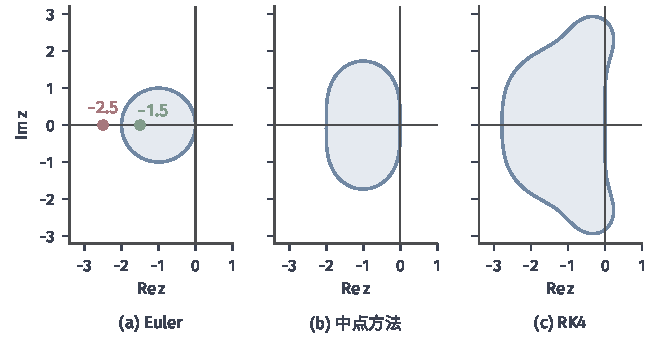
\includegraphics[width=112mm]{figures/06-differential-equations/01-ordinary-differential-equations/matplotlib/odenum-stability-explicit/figure.pdf}
 \caption{显式方法的绝对稳定域（浅蓝），边界是$\lvert R(z)\rvert=1$，三幅图的坐标范围相同。(a)显式Euler方法，红点$z=-2.5$在域外，绿点$z=-1.5$在域内；(b)中点方法，实轴上止于$-2$；(c)RK4，实轴上止于约$-2.785$。}
 \label{fig:odenum-stability-explicit}
\end{BookInlineFigure}

阶数提高，稳定域略有扩大，但RK4的实轴范围也只到约$-2.785$。原因在结构上：显式Runge--Kutta方法的$R(z)$总是多项式，当$\lvert z\rvert\to\infty$时$\lvert R(z)\rvert\to\infty$，所以稳定域必定有界。高阶的显式方法解除不了刚性带来的限制。

\paragraph{这一分析能说明什么}
测试方程分析的是数值扰动怎样传播，适用的情形是线性、常系数、矩阵可对角化，并且步长固定。在非线性问题上，通常把$\partial_{\bm{x}}\bm{f}$沿解冻结在某一时刻来做估计，这只是启发式的做法。它不能代替第~\ref{sec:odenum-error-convergence}节那样的收敛论证。

下面的时变系统说明冻结的特征值可能误导人。取矩阵
\[
 \bm{A}(t)=\begin{bmatrix}
  -1+\tfrac{3}{2}\cos^2t & 1-\tfrac{3}{2}\sin t\cos t\\
  -1-\tfrac{3}{2}\sin t\cos t & -1+\tfrac{3}{2}\sin^2t
 \end{bmatrix}.
\]
它的迹恒为$-1/2$，行列式恒为$1/2$，所以每个时刻的特征值都是$(-1\pm\mathrm{i}\sqrt{7})/4$，实部为$-1/4$，全在左半平面。

可是直接代入可以验证，下面的函数是方程$\dot{\bm{x}}=\bm{A}(t)\bm{x}$的解：
\[
 \bm{x}(t)=\mathrm{e}^{t/2}\begin{bmatrix}\cos t\\-\sin t\end{bmatrix},
\]
它的长度按$\mathrm{e}^{t/2}$增长（图~\ref{fig:odenum-frozen-coefficients}）。每一时刻看起来都是衰减的，解却在增长，因为特征方向在随时间转动。

\begin{BookInlineFigure}
 \centering
 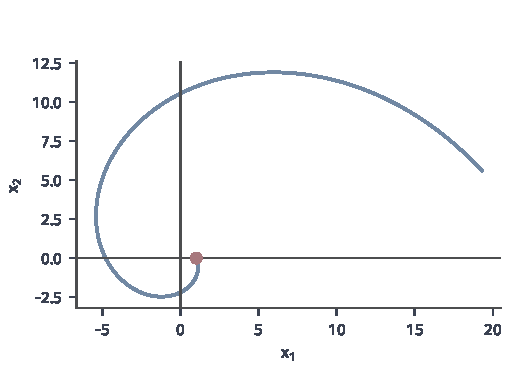
\includegraphics[width=86mm]{figures/06-differential-equations/01-ordinary-differential-equations/matplotlib/odenum-frozen-coefficients/figure.pdf}
 \caption{冻结特征值全在左半平面的时变线性系统。蓝线是从红点$(1,0)$出发的解，在$t\in[0,6]$上按$\mathrm{e}^{t/2}$向外旋转。}
 \label{fig:odenum-frozen-coefficients}
\end{BookInlineFigure}

\begin{BookInlineTable}
 \centering
 \caption{收敛与绝对稳定性的对比。}
 \label{tab:odenum-convergence-stability}
 \begin{tabular}{lll}
  \toprule
  & 收敛（定理~\ref{thm:odenum-global-error}） & 绝对稳定性\\
  \midrule
  关心的极限 & 固定$T$，$h\to0$ & 固定$h$，步数增加\\
  适用问题 & 非线性，有限区间 & 线性测试方程\\
  回答的问题 & 误差怎样随$h$减小 & 扰动是否放大\\
  \bottomrule
 \end{tabular}
\end{BookInlineTable}

\subsection{隐式格式}
\label{sec:odenum-implicit}

显式方法的放大因子是多项式，稳定域有界。要让稳定域覆盖整个左半平面，$R(z)$必须换成有理函数，这要求更新式的右端用到未知的新值。

\paragraph{主要思想}
回到积分式~\eqref{eq:odenum-integral-step}。Euler方法用左端点的值近似被积函数，现在改用右端点的值，得到\term{后向Euler方法}（backward Euler method）：
\begin{equation}
 \bm{x}^{(k+1)}=\bm{x}^{(k)}+h\,\bm{f}\bigl(t_{k+1},\bm{x}^{(k+1)}\bigr).
 \label{eq:odenum-backward-euler}
\end{equation}
未知的$\bm{x}^{(k+1)}$出现在等式两边，每一步都要解一个方程，这样的方法称为\term{隐式方法}（implicit method）。

把左右两端点的值平均，得到\term{梯形方法}（trapezoidal rule）：
\begin{equation}
 \bm{x}^{(k+1)}=\bm{x}^{(k)}+\frac{h}{2}\Bigl(\bm{f}\bigl(t_k,\bm{x}^{(k)}\bigr)+\bm{f}\bigl(t_{k+1},\bm{x}^{(k+1)}\bigr)\Bigr).
 \label{eq:odenum-trapezoid}
\end{equation}

在非刚性问题上它们的局部误差可以直接估计。对后向Euler方法，设$\bm{x}\in C^2$，$hL<1$，$\bm{y}=\bm{\Psi}_h(t_k,\bm{x}(t_k))$。真解满足同一个方程，只多一个余项$\bm{r}$，其大小满足
\[
 \lVert\bm{r}\rVert_2\leq\frac{h^2}{2}\max_{t}\lVert\ddot{\bm{x}}(t)\rVert_2.
\]
两式相减得到
\[
 \lVert\bm{y}-\bm{x}(t_{k+1})\rVert_2\leq hL\lVert\bm{y}-\bm{x}(t_{k+1})\rVert_2+\lVert\bm{r}\rVert_2,
\]
移项得到
\[
 \bigl\lVert\bm{\ell}^{(k+1)}\bigr\rVert_2\leq\frac{\lVert\bm{r}\rVert_2}{1-hL},
\]
所以后向Euler方法的阶是$1$。

梯形方法的阶是$2$，要求$\bm{x}\in C^3$：梯形求积公式的余项是$O(h^3)$，推导方式相同。这里的估计用了$hL<1$，刚性问题的$hL$很大，上面的估计就失去了意义，要靠下面的稳定性分析。

\paragraph{放大因子与稳定域}
把后向Euler方法用于测试方程，得到$x^{(k+1)}=x^{(k)}+zx^{(k+1)}$，解出
\begin{equation}
 R(z)=\frac{1}{1-z}.
 \label{eq:odenum-be-factor}
\end{equation}
于是$\lvert R(z)\rvert\leq1$等价于$\lvert1-z\rvert\geq1$，稳定域是以$1$为心的单位开圆盘的外部。

对梯形方法，同样的计算给出
\begin{equation}
 R(z)=\frac{1+z/2}{1-z/2}.
 \label{eq:odenum-trapezoid-factor}
\end{equation}
直接展开两个模的平方可得
\[
 \lvert1+z/2\rvert^2-\lvert1-z/2\rvert^2=2\,\mathrm{Re}\,z,
\]
所以$\lvert R(z)\rvert\leq1$恰好等价于$\mathrm{Re}\,z\leq0$，稳定域就是闭左半平面（图~\ref{fig:odenum-stability-implicit}）。

\begin{BookInlineFigure}
 \centering
 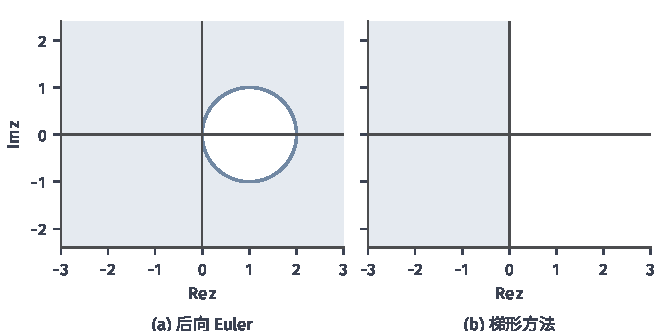
\includegraphics[width=112mm]{figures/06-differential-equations/01-ordinary-differential-equations/matplotlib/odenum-stability-implicit/figure.pdf}
 \caption{隐式方法的绝对稳定域（浅蓝）。(a)后向Euler方法，稳定域是以$1$为心的单位开圆盘（白色）的外部；(b)梯形方法，稳定域恰为闭左半平面。两者都包含闭左半平面，图中只画出有限范围。}
 \label{fig:odenum-stability-implicit}
\end{BookInlineFigure}

若稳定域包含闭左半平面，就称方法\term{A稳定}（A-stable）。这两个隐式方法都是A稳定的，因此用于系统~\eqref{eq:odenum-stiff-system}时不论$h$多大，线性模式都不会被放大。

\paragraph{快速模式的数值阻尼}
A稳定只保证不放大，不保证快速模式被迅速消除。比较$z\to-\infty$时的极限：真解的因子$\mathrm{e}^{z}\to0$，后向Euler的$R(z)\to0$，梯形方法的$R(z)\to-1$（图~\ref{fig:odenum-amplification-real}）。

\begin{BookInlineFigure}
 \centering
 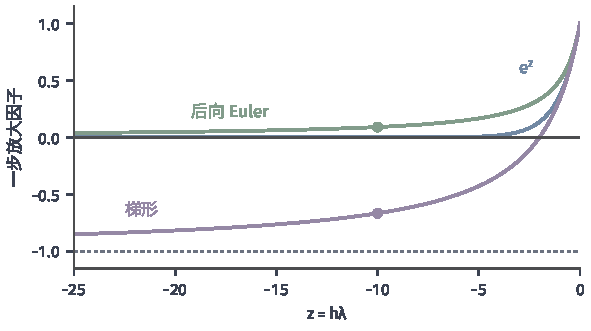
\includegraphics[width=100mm]{figures/06-differential-equations/01-ordinary-differential-equations/matplotlib/odenum-amplification-real/figure.pdf}
 \caption{负实轴上的一步放大因子。蓝线是真解的$\mathrm{e}^{z}$，绿线是后向Euler的$1/(1-z)$，紫线是梯形方法的$(1+z/2)/(1-z/2)$，灰色虚线是$-1$。圆点标出$z=-10$处的取值$1/11$和$-2/3$。}
 \label{fig:odenum-amplification-real}
\end{BookInlineFigure}

后向Euler对快速模式有很强的\term{数值阻尼}（numerical damping），模式一步就几乎消失。梯形方法的快速模式几乎不衰减，只是每步变号。在$z=-10$时，后向Euler的因子是$1/11$，梯形方法是$-2/3$。若方法既A稳定又满足$\lim_{z\to-\infty}R(z)=0$，就称方法\term{L稳定}（L-stable），后向Euler是，梯形方法不是。

\paragraph{计算过程：线性系统}
线性系统$\dot{\bm{x}}=\bm{A}\bm{x}$上，后向Euler方法每步解一个线性方程组，结果可以写成显式形式：
\begin{equation}
 \bm{x}^{(k+1)}=(\bm{I}-h\bm{A})^{-1}\bm{x}^{(k)}.
 \label{eq:odenum-be-linear}
\end{equation}
实际计算不求逆，而是分解一次$\bm{I}-h\bm{A}$再反复回代，步长不变时每步只需回代。下面用系统~\eqref{eq:odenum-stiff-system}演示，取$h=0.2$，它是显式方法上限$0.04$的五倍。

\needspace{6\baselineskip}
\paragraph{变量}
\begin{itemize}
 \item $\bm{x}^{(k)}\in\mathbb{R}^{n}$：第$k$个网格点的数值解。
 \item $\bm{I}-h\bm{A}\in\mathbb{R}^{n\times n}$：每步的系数矩阵，步长不变时只分解一次。
\end{itemize}

\paragraph{初始化}
把数值解初始化为初值，并构造系数矩阵。例中
\[
 \bm{x}^{(0)}=\begin{bmatrix}1\\0\end{bmatrix},\qquad
 \bm{I}-h\bm{A}=\begin{bmatrix}1.2&0\\-10&11\end{bmatrix}.
\]

\needspace{6\baselineskip}
\paragraph{每轮更新}
对$k=0,1,\ldots,N-1$依次执行：
\begin{enumerate}
 \item \textbf{求解第一个分量。}例中系数矩阵是下三角的，由第一行得到
 \[
  x_1^{(k+1)}=\frac{x_1^{(k)}}{1+h}.
 \]
 例中第一轮
 \[
  x_1^{(1)}=\frac{1}{1.2}=0.833333.
 \]
 \item \textbf{求解第二个分量。}由第二行得到
 \[
  x_2^{(k+1)}=\frac{x_2^{(k)}+50h\,x_1^{(k+1)}}{1+50h}.
 \]
 例中第一轮
 \[
  x_2^{(1)}=\frac{0+10\times0.833333}{11}=0.757576.
 \]
 例中第二轮，两个分量依次为
 \[
  x_1^{(2)}=0.694444,\qquad x_2^{(2)}=\frac{0.757576+6.944444}{11}=0.700184.
 \]
 \item \textbf{停止。}走满$N$步后结束。
\end{enumerate}
最终例中$t=0.4$处$x_2^{(2)}=0.700184$，真值约为$0.684000$，没有振荡。第一步的误差较大，因为$h=0.2$完全跨过了快速过渡，这是用一步盖过快速过程的代价，后面的步很快贴回真解。

图~\ref{fig:odenum-implicit-stiff}比较两种隐式方法。梯形方法的第一轮为
\[
 x_2^{(1)}=\frac{5\,(x_1^{(0)}+x_1^{(1)})-4\,x_2^{(0)}}{6}=1.515152,
\]
其中$x_1^{(1)}=0.818182$。它明显越过真解，之后按因子$-2/3$交替变号衰减，正好体现了图~\ref{fig:odenum-amplification-real}中$z=-10$处的差别。

\begin{BookInlineFigure}
 \centering
 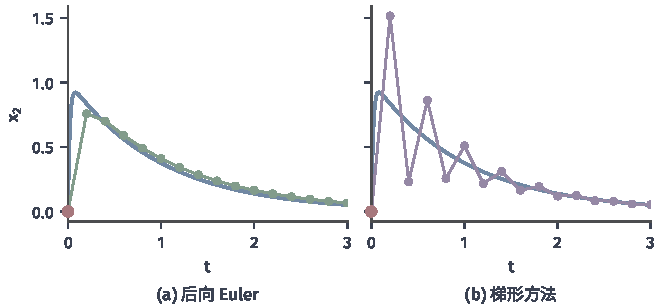
\includegraphics[width=112mm]{figures/06-differential-equations/01-ordinary-differential-equations/matplotlib/odenum-implicit-stiff/figure.pdf}
 \caption{隐式方法用于系统~\eqref{eq:odenum-stiff-system}，$h=0.2$，纵轴为$x_2$。蓝线是真解，红点是初值。(a)后向Euler方法（绿）没有振荡；(b)梯形方法（紫）第一步越过真解，之后交替变号衰减。}
 \label{fig:odenum-implicit-stiff}
\end{BookInlineFigure}

\paragraph{计算过程：非线性方程}
非线性问题的隐式更新没有闭式，需要迭代。对后向Euler方法，设$\bm{y}$是要求的$\bm{x}^{(k+1)}$，解方程
\begin{equation}
 \bm{G}(\bm{y})=\bm{y}-\bm{x}^{(k)}-h\,\bm{f}(t_{k+1},\bm{y})=\bm{0}.
 \label{eq:odenum-implicit-equation}
\end{equation}

最直接的不动点迭代$\bm{y}\leftarrow\bm{x}^{(k)}+h\bm{f}(t_{k+1},\bm{y})$只在$hL<1$时保证压缩，这恰好是显式方法的步长量级，隐式方法的好处就丢掉了。所以刚性问题通常用Newton迭代，即每次解线性方程组
\[
 \bigl(\bm{I}-h\,\partial_{\bm{x}}\bm{f}(t_{k+1},\bm{y})\bigr)\bm{\Delta}=-\bm{G}(\bm{y}),
\]
再令$\bm{y}\leftarrow\bm{y}+\bm{\Delta}$。Newton法的收敛性质可参考\BookChapterRef{chap:second-order-methods}{卷五第7章“二阶方法”}，线性方程组的分解可参考\BookChapterRef{chap:direct-linear-solvers}{卷二第12章“线性方程的直接求解”}。

用例~\eqref{eq:odenum-running}演示，$h=0.5$。一维时
\[
 G(y)=y-x^{(k)}-0.5\,y(1-y),\qquad G'(y)=1-0.5(1-2y).
\]
以显式Euler的结果$y=0.28$作初值，第一步的迭代为
\[
 G(0.28)=-0.0208,\quad G'(0.28)=0.78,\quad y=0.306667.
\]
第二次迭代得到
\[
 G(0.306667)=3.56\times10^{-4},\quad G'(0.306667)=0.806667,\quad y=0.306226.
\]
此时$\lvert G\rvert$已降到$10^{-7}$量级，取$x^{(1)}=0.306226$。

\paragraph{内部容差计入误差预算}
隐式更新解不到严格的零。迭代提前停止留下的偏差，正是式~\eqref{eq:odenum-computed}中的计算误差$\bm{\delta}^{(k+1)}$。由定理~\ref{thm:odenum-global-error}，它在全局误差中贡献$\varepsilon/h$的量级。

图~\ref{fig:odenum-inner-tolerance}给出一个实验：对例~\eqref{eq:odenum-running}用梯形方法，内部用不动点迭代（此处$h$较小，迭代是压缩的），当相邻两次迭代之差不超过内部容差时停止。容差很小时，误差停在由截断决定的平台；容差放松到一定程度，误差会阶梯式上升，最宽松时一次迭代就停，格式退化为一阶。

\begin{BookInlineFigure}
 \centering
 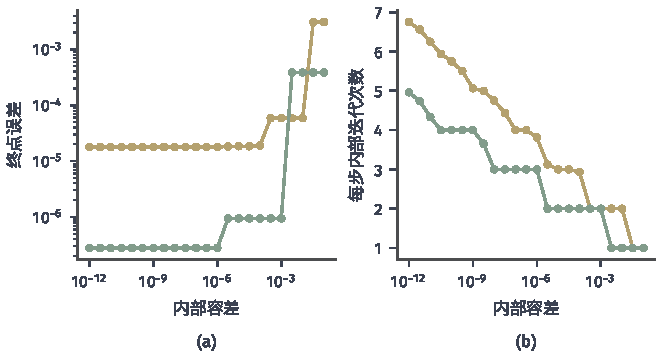
\includegraphics[width=112mm]{figures/06-differential-equations/01-ordinary-differential-equations/matplotlib/odenum-inner-tolerance/figure.pdf}
 \caption{内部方程的容差对梯形方法的影响，问题为式~\eqref{eq:odenum-running}，$T=1$，内部采用不动点迭代。黄线$N=16$，绿线$N=128$。(a)终点误差：容差小时不随容差变化，容差大时误差阶梯式上升。(b)每步平均内部迭代次数：容差越小迭代越多。}
 \label{fig:odenum-inner-tolerance}
\end{BookInlineFigure}

这个实验给出的预算原则是：内部容差要明显小于这一步允许的局部误差，否则花在高阶公式上的计算会被内部误差抵消；反过来把容差压得远低于截断误差，只是白白增加迭代次数。

\paragraph{不能只看阶数}
选择方法时要同时考虑稳定域、每步求解代价和计算误差。对系统~\eqref{eq:odenum-stiff-system}，RK4虽然是四阶，步长仍受$2.785/50\approx0.056$的限制，走到$T=4$至少$72$步、$288$次右端求值。一阶的后向Euler方法取$h=0.2$只需$20$步，每步解一次$2\times2$的线性方程组，而且不会发散。

反过来，方程若不刚性，隐式方法每步要解方程，就比显式方法贵得多，也得不到额外好处。表~\ref{tab:odenum-implicit-compare}汇总本节的方法。

\begin{BookInlineTable}
 \centering
 \caption{显式与隐式方法的对比，$z=h\lambda$。}
 \label{tab:odenum-implicit-compare}
 \begin{tabular}{llcc}
  \toprule
  方法 & $R(z)$ & 阶 & A稳定\\
  \midrule
  显式Euler & $1+z$ & 1 & 否\\
  RK4 & 四次多项式 & 4 & 否\\
  后向Euler & $1/(1-z)$ & 1 & 是，$R(-\infty)=0$\\
  梯形 & $(1+z/2)/(1-z/2)$ & 2 & 是，$R(-\infty)=-1$\\
  \bottomrule
 \end{tabular}
\end{BookInlineTable}


\section{自适应步长}
\label{sec:odenum-adaptive}

固定步长要在全程迁就最难走的一段。解在某处急转，别处平缓，均匀的小步长就是浪费，均匀的大步长又不够准。程序能不能边走边判断，自己决定每一步走多远？

\paragraph{主要思想：估计局部误差}
要调节步长，先要知道这一步的误差有多大。真解未知，但可以用两个不同精度的结果相减来估计。

一种办法是\term{步长加倍}（step doubling）。设方法的阶为$p$，从同一点出发，用步长$h$走一步得到$\bm{y}_1$，用步长$h/2$走两步得到$\bm{y}_2$。忽略高阶项，两者的误差主要部分分别是$\bm{c}h^{p+1}$和$2\bm{c}(h/2)^{p+1}$，相减消去未知的真解，得到对$\bm{y}_2$的误差估计
\begin{equation}
 \bm{x}(t+h)-\bm{y}_2\approx\frac{\bm{y}_2-\bm{y}_1}{2^{p}-1}.
 \label{eq:odenum-step-doubling}
\end{equation}

例~\eqref{eq:odenum-running}的第一步，Euler方法用$h=0.5$得$0.28$，用两个$0.25$的半步得$0.2856$，由式~\eqref{eq:odenum-step-doubling}估计真解比$0.2856$约大$0.0056$。实际差是$0.291875-0.2856=0.0063$，估计相当准确。这种做法要多算一倍的步，代价偏高。

另一种办法用同一组阶段斜率组合出两个不同阶的结果，它们的差就是误差估计，不增加右端求值，这样的方法称为\term{嵌入式Runge--Kutta方法}（embedded Runge--Kutta method）。最简单的例子是Heun--Euler对。

取Heun方法的两个斜率$\bm{k}_1=\bm{f}(t,\bm{x})$，$\bm{k}_2=\bm{f}(t+h,\bm{x}+h\bm{k}_1)$。一阶的结果只用$\bm{k}_1$，二阶的结果用两者平均：
\[
 \bm{x}_{\mathrm{low}}=\bm{x}+h\bm{k}_1,\qquad
 \bm{x}_{\mathrm{high}}=\bm{x}+\frac{h}{2}(\bm{k}_1+\bm{k}_2).
\]
两者之差估计低阶结果的误差：
\begin{equation}
 \bm{d}=\bm{x}_{\mathrm{high}}-\bm{x}_{\mathrm{low}}=\frac{h}{2}(\bm{k}_2-\bm{k}_1).
 \label{eq:odenum-embedded-estimate}
\end{equation}
实际使用的是更高阶的配对，例如Dormand--Prince的五四阶方法\scite{math-hairer1993ode}，原理相同。

\paragraph{主要思想：尺度、接受与新步长}
误差估计要和一个容许的尺度比较。各分量量纲可能不同，大小也可能相差很多，所以给每个分量一个尺度，同时用\term{绝对容差}（absolute tolerance）$\eta_{\mathrm{a}}$和\term{相对容差}（relative tolerance）$\eta_{\mathrm{r}}$：
\begin{equation}
 w_i=\eta_{\mathrm{a}}+\eta_{\mathrm{r}}\max\bigl\{\lvert x_i\rvert,\ \lvert x_{\mathrm{high},i}\rvert\bigr\}.
 \label{eq:odenum-scale}
\end{equation}
相对容差让大分量按比例控制精度；绝对容差防止分量接近零时尺度也趋于零，把步长压到不合理的小。

归一化的误差取各分量比值的最大值：
\begin{equation}
 \mathrm{err}=\max_{i}\frac{\lvert d_i\rvert}{w_i}.
 \label{eq:odenum-err}
\end{equation}
若$\mathrm{err}\leq1$，这一步被接受，否则放弃这一步，用更小的步长重算。

无论接受与否，都要决定下一个步长。低阶结果的阶为$q$时，$\mathrm{err}$大约正比于$h^{q+1}$，要让它变成$1$，步长应乘以$\mathrm{err}^{-1/(q+1)}$。加上安全系数$\gamma<1$和增减幅度的限制，得到
\begin{equation}
 h_{\mathrm{new}}=h\,\min\Bigl\{f_{\max},\ \max\bigl\{f_{\min},\ \gamma\,\mathrm{err}^{-1/(q+1)}\bigr\}\Bigr\}.
 \label{eq:odenum-step-control}
\end{equation}
限制幅度是因为$\mathrm{err}$只是估计，步长剧烈变化会使估计失效。

\paragraph{计算过程}
下面用例~\eqref{eq:odenum-running}演示Heun--Euler对，$q=1$，取容差和控制参数为
\[
 \eta_{\mathrm{a}}=\eta_{\mathrm{r}}=10^{-3},\quad\gamma=0.9,\quad f_{\min}=0.2,\quad f_{\max}=5,
\]
初始步长取$h=0.5$，积分到$T=1$，接受后沿用高阶结果继续。

\needspace{6\baselineskip}
\paragraph{变量}
\begin{itemize}
 \item $t$，$\bm{x}\in\mathbb{R}^{n}$：已接受的当前时刻和数值解。
 \item $h$：当前尝试的步长。
 \item $\bm{k}_1,\bm{k}_2\in\mathbb{R}^{n}$：本次尝试的两个阶段斜率。
 \item $\bm{d}$，$\mathrm{err}$：误差估计和归一化误差。
 \item 标记$\mathrm{failed}$：上一次尝试是否被拒绝，被拒绝后下一步的$f_{\max}$取$1$，避免紧接着又放大步长。
\end{itemize}

\paragraph{初始化}
把当前点初始化为初值，并设初始步长。例中
\[
 t=0,\qquad x=0.2,\qquad h=0.5,\qquad \mathrm{failed}=\text{否}.
\]

\needspace{6\baselineskip}
\paragraph{每轮更新}
当$t<T$时重复：
\begin{enumerate}

 \item \textbf{截断到终点。}令$h\leftarrow\min\{h,T-t\}$，保证不越过$T$。

 \item \textbf{算两个斜率和两个结果。}计算$\bm{k}_1,\bm{k}_2$，$\bm{x}_{\mathrm{high}}$，并由式~\eqref{eq:odenum-embedded-estimate}算$\bm{d}$。例中第一次尝试
 \[
  k_1=0.16,\qquad k_2=f(0.28)=0.2016,
 \]
 于是
 \[
  x_{\mathrm{high}}=0.2904,\qquad d=0.25\times0.0416=0.0104.
 \]

 \item \textbf{比较尺度。}由式~\eqref{eq:odenum-scale}和式~\eqref{eq:odenum-err}计算$\mathrm{err}$。例中第一次尝试
 \[
  w=10^{-3}+10^{-3}\times0.2904=0.00129,\qquad \mathrm{err}=8.06.
 \]

 \item \textbf{接受或拒绝。}若$\mathrm{err}\leq1$，令$t\leftarrow t+h$，$\bm{x}\leftarrow\bm{x}_{\mathrm{high}}$，$\mathrm{failed}$置为否；否则状态不变，$\mathrm{failed}$置为是。例中第一次$\mathrm{err}>1$，拒绝，状态仍为$(0,\,0.2)$。

 \item \textbf{更新步长。}由式~\eqref{eq:odenum-step-control}计算$h_{\mathrm{new}}$，令$h\leftarrow h_{\mathrm{new}}$。例中第一次尝试
 \[
  h_{\mathrm{new}}=0.5\times\max\bigl\{0.2,\ 0.9\times8.06^{-1/2}\bigr\}=0.5\times0.317=0.1585.
 \]
 例中第二次尝试用$h=0.1585$，得到
 \[
  k_2=0.174574,\qquad x_{\mathrm{high}}=0.226517,\qquad \mathrm{err}=0.942,
 \]
 这一步被接受，$t$更新为$0.1585$，$x$更新为$0.226517$。

 \item \textbf{停止。}当$t=T$时结束。
\end{enumerate}
全程的尝试列于表~\ref{tab:odenum-adaptive-trace}。一共$8$次尝试、$16$次右端求值，一次被拒绝；最终$x=0.404269$，真值$0.404610$，全局误差$-3.4\times10^{-4}$。

\begin{BookInlineTable}
 \centering
 \caption{Heun--Euler对在式~\eqref{eq:odenum-running}上的步长控制，$\eta_{\mathrm{a}}=\eta_{\mathrm{r}}=10^{-3}$。最后一步被截断以恰好到达$T=1$。}
 \label{tab:odenum-adaptive-trace}
 \begin{tabular}{rrrrc}
  \toprule
  $t$ & $h$ & $x_{\mathrm{high}}$ & $\mathrm{err}$ & 结果\\
  \midrule
  0 & 0.50000 & 0.290400 & 8.060 & 拒绝\\
  0 & 0.15851 & 0.226517 & 0.942 & 接受\\
  0.15851 & 0.14701 & 0.253260 & 0.787 & 接受\\
  0.30552 & 0.14911 & 0.282437 & 0.763 & 接受\\
  0.45462 & 0.15366 & 0.314545 & 0.735 & 接受\\
  0.60828 & 0.16128 & 0.350259 & 0.698 & 接受\\
  0.76956 & 0.17373 & 0.390689 & 0.642 & 接受\\
  0.94329 & 0.05671 & 0.404269 & 0.056 & 接受\\
  \bottomrule
 \end{tabular}
\end{BookInlineTable}

\paragraph{步长怎样跟随解}
图~\ref{fig:odenum-adaptive-steps}是同一控制器用在变化更剧烈的方程$\dot{x}=12x(1-x)$上的结果，$x(0)=0.02$，容差仍为$10^{-3}$。解从缓慢上升到快速爬升，再到贴近平衡点。控制器在曲线转弯的区域用小步，在平衡点附近把步长放大，共接受$49$步、拒绝$6$步，$110$次右端求值，终点误差约$5\times10^{-4}$。

\begin{BookInlineFigure}
 \centering
 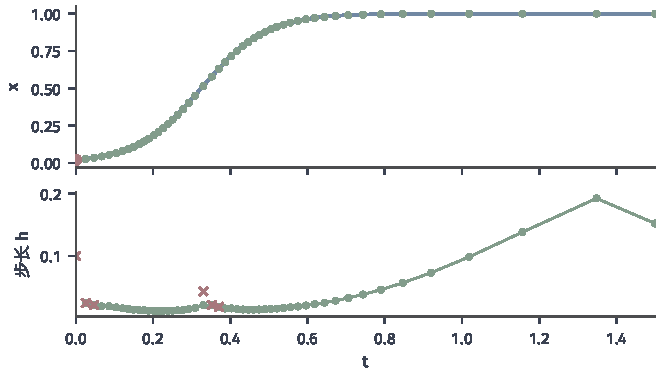
\includegraphics[width=112mm]{figures/06-differential-equations/01-ordinary-differential-equations/matplotlib/odenum-adaptive-steps/figure.pdf}
 \caption{自适应步长跟随解的变化，方程$\dot{x}=12x(1-x)$，$x(0)=0.02$，$\eta_{\mathrm{a}}=\eta_{\mathrm{r}}=10^{-3}$。上图蓝线是真解，红点是初值，绿点是接受的网格值；下图绿线是接受步的步长，红叉是被拒绝的尝试。}
 \label{fig:odenum-adaptive-steps}
\end{BookInlineFigure}

\paragraph{局部容差不直接保证全局精度}
控制器管的是每一步新增的偏差，全局误差还要乘上流映射的放大。回到第~\ref{sec:odenum-time-discretization}节的方程$\dot{x}=\sigma(x-\cos t)-\sin t$，$x(0)=1$，积分到$T=2$。图~\ref{fig:odenum-adaptive-global}显示，同样的局部容差，$\sigma=-5$时全局误差大致等于容差，$\sigma=5$时放大了四个多数量级。容差取$10^{-5}$时，前者的全局误差约$6\times10^{-6}$，后者约$0.18$。

\begin{BookInlineFigure}
 \centering
 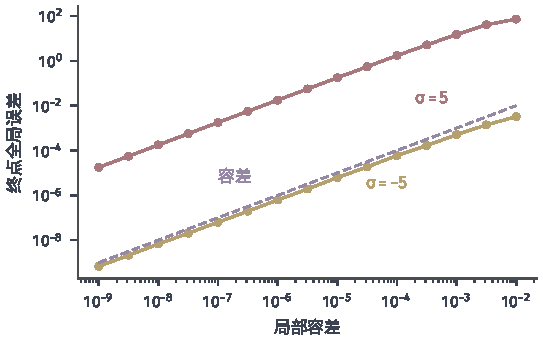
\includegraphics[width=92mm]{figures/06-differential-equations/01-ordinary-differential-equations/matplotlib/odenum-adaptive-global/figure.pdf}
 \caption{局部容差与终点全局误差，方程为$\dot{x}=\sigma(x-\cos t)-\sin t$，$x(0)=1$，$T=2$，$\eta_{\mathrm{a}}=\eta_{\mathrm{r}}$。黄线$\sigma=-5$，红线$\sigma=5$，紫色虚线为容差本身。}
 \label{fig:odenum-adaptive-global}
\end{BookInlineFigure}

所以容差不是全局精度的保证。可靠的做法是把容差减小一两个数量级再解一次，比较两次的结果；或者用第~\ref{chap:ode-sensitivity}章的敏感性信息估计放大因子。这样的比较检验的是数值误差，并不能发现模型本身的错误。

\paragraph{自适应不能解决刚性}
控制器还会被稳定性牵着走。把Heun--Euler对用于系统~\eqref{eq:odenum-stiff-system}，容差$10^{-3}$，走到$T=4$。快速过渡结束后，解已经很平缓，局部误差估计却不断地“被激发”：一旦步长越过稳定上限，快速模式开始放大，误差估计变大，步长又被压回来。

结果是步长一直贴着上限$2/50$上下摆动（图~\ref{fig:odenum-adaptive-stiff}）。共接受$141$步、拒绝$13$步，$308$次右端求值，后半程的平均步长约$0.039$，而精度本来允许走得更远。

\begin{BookInlineFigure}
 \centering
 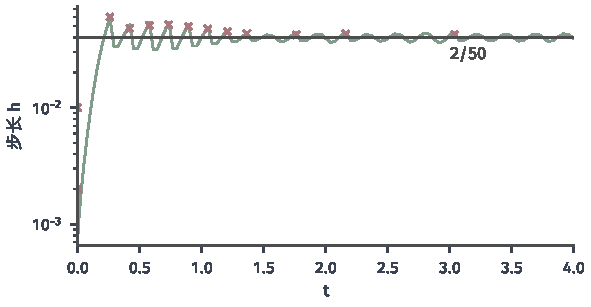
\includegraphics[width=100mm]{figures/06-differential-equations/01-ordinary-differential-equations/matplotlib/odenum-adaptive-stiff/figure.pdf}
 \caption{显式嵌入对用于刚性系统~\eqref{eq:odenum-stiff-system}时的步长历史，容差$10^{-3}$。绿线是接受步的步长，红叉是被拒绝的尝试，深灰线是稳定上限$2/50$。解变平缓之后，步长仍被稳定性限制。}
 \label{fig:odenum-adaptive-stiff}
\end{BookInlineFigure}

步长长期贴着一个与解的光滑程度无关的水平，同时反复被拒绝，这本身就是刚性的信号，应当换成隐式方法。求值次数的增长同样值得监控：它比预期多很多时，要么是方程刚性，要么是右端有不连续点，控制器把步长压小只是在逼近那一点，并不能恢复方法的阶。


\section{本章小结}
\label{sec:odenum-summary}

本章回答了开头的三个问题。怎样走一步：所有方法都在近似积分式~\eqref{eq:odenum-integral-step}，显式Euler方法只看起点，Runge--Kutta方法在一步内多次采样并匹配Taylor展开，隐式方法把未知的终点也放进来。

误差怎样累积：局部截断误差沿真解定义，没有除以步长。定理~\ref{thm:odenum-global-error}说明，在解存在的有限区间上，只要方法一步稳定、一步误差一致地是$O(h^{p+1})$、初值误差和计算误差足够小，全局误差就是$O(h^{p})$。它的常数含有$\mathrm{e}^{\Lambda T}$，这是有限时间的结论，不描述长期行为。

步长由什么决定：非刚性问题由精度决定，刚性问题由稳定性决定。绝对稳定域回答固定步长下扰动是否放大，它基于线性测试方程，不能代替一般的收敛论证。

表~\ref{tab:odenum-choice}按问题的特点比较代表方法。

\begin{BookInlineTable}
 \centering
 \caption{方法选择的对比。}
 \label{tab:odenum-choice}
 \begin{tabular}{p{28mm}p{30mm}p{36mm}}
  \toprule
  问题特点 & 适用方法 & 主要代价或风险\\
  \midrule
  光滑，非刚性，低精度 & 低阶显式方法 & 精度要求提高时成本急增\\
  光滑，非刚性，高精度 & RK4或高阶嵌入对 & 需要足够的光滑性\\
  右端有已知跳变 & 在跳变点分段积分 & 不分段时阶数丢失\\
  刚性 & 后向Euler等隐式方法 & 每步解方程，内部容差计入预算\\
  解的尺度变化大 & 自适应步长 & 容差不等于全局精度\\
  \bottomrule
 \end{tabular}
\end{BookInlineTable}

两种常用的检验要分清。步长细化比较不同步长的结果，能观察实际的收敛阶，发现阶数丢失和舍入误差主导，但要求解在相应步长上已进入渐近范围。局部误差估计只度量一步新增的偏差，不包含累积，也察觉不到系统性的模型错误。

偏微分方程在空间离散后成为大型常微分方程组，时间推进可以直接使用本章的方法，空间网格越细，系统通常越刚性，具体分析见第~\ref{chap:pde-numerical-methods}章。长时间积分时的结构保持、吸引子等离散动力学问题超出了有限区间收敛定理的范围，可参考\BookChapterRef{chap:dynamical-systems-long-term}{卷九第1章“动力系统与轨迹的长期行为”}。

